\begin{chapterpage}{Summarizing data}
  \chaptertitle{Summarizing data}
  \label{summarizingData}
  \label{ch_summarizing_data}
  \chaptersection{numericalData}
  \chaptersection{categoricalData}
  \chaptersection{caseStudyMalariaVaccine}
\end{chapterpage}
\renewcommand{\chapterfolder}{ch_summarizing_data}

\chapterintro{This chapter focuses on the mechanics
  and construction of summary statistics and graphs.
  In practice, we use statistical software for generating
  most of the summaries and graphs presented in this chapter.
  However since this might be your first exposure to these
  concepts, we take our time in this chapter to detail
  how to compute them.
  Mastery of the content presented in this chapter
  will be crucial for understanding the methods and
  techniques introduced in future chapters of the book.}



%%%%%
\section{Examining numerical data}
\label{numericalData}

% library(openintro); ind <- c(1:5, 50); d <- loan50$interest_rate; (m <- round(mean(d), 2)); d[ind]; (dev <- d - m)[ind]; (dev2 <- dev^2)[ind]; (s2 <- sum(dev2) / 49); (s <- sqrt(s2)); var(d); sd(d); median(d); IQR(d); quantile(d, c(0.25, 0.75))
\newcommand{\loanA}{10.90}
\newcommand{\loanB}{9.92}
\newcommand{\loanC}{26.30}
\newcommand{\loanD}{9.92}
\newcommand{\loanY}{9.43}
\newcommand{\loanZ}{6.08}
\newcommand{\loanAvg}{11.57}
\newcommand{\loanVar}{25.52}
\newcommand{\loanSD}{5.05}
\newcommand{\loanN}{50}
\newcommand{\loanMedianBelow}{9.93\%}
\newcommand{\loanMedianAbove}{9.93\%}
\newcommand{\loanMedian}{9.93\%}
\newcommand{\loanQA}{7.96}
\newcommand{\loanQC}{13.72}
\newcommand{\loanIQR}{5.76}
\newcommand{\loanAdev}{-0.67}
\newcommand{\loanBdev}{-1.65}
\newcommand{\loanCdev}{14.73}
\newcommand{\loanDdev}{-1.65}
\newcommand{\loanYdev}{-2.14}
\newcommand{\loanZdev}{-5.49}
\newcommand{\loanSmallestValue}{5.31}
\newcommand{\loanLargestValue}{26.30}


In this section we will explore techniques for
summarizing numerical variables.
For example, consider the \var{loan\us{}amount} variable
from the \data{loan50} data set, which represents the loan
size for all 50 loans in the data set.
This variable is numerical since we can sensibly discuss
the numerical difference of the size of two loans.
On the other hand, area codes and zip codes are not numerical,
but rather they are categorical variables.

Throughout this section and the next, we will apply these
methods using the \data{loan50} and \data{county} data sets,
which were introduced in Section~\ref{dataBasics}.
If you'd like to review the variables from either data set,
see pages~\ref{loan50DF} and~\ref{countyDF}.


\subsection{Scatterplots for paired data}
\label{scatterPlots}

\index{data!loan50|(}

A \term{scatterplot} provides a case-by-case view of data
for two numerical variables.
In Figure~\ref{multiunitsVsOwnership} on
page~\pageref{multiunitsVsOwnership}, a scatterplot
was used to examine the homeownership rate against
the fraction of housing units that were part of
multi-unit properties
(e.g. apartments) in the \data{county} data set.
Another scatterplot is shown in Figure~\ref{loan50_amt_vs_income},
comparing the total income of a borrower
(\var{total\us{}income}) and the amount they borrowed
(\var{loan\us{}amount}) for the \data{loan50} data set.
In any scatterplot, each point represents a single case.
Since there are \loanN{} cases in \data{loan50},
there are \loanN{} points in Figure~\ref{loan50_amt_vs_income}.

\begin{figure}[h]
  \centering
  \Figure{0.8}{loan50_amt_vs_income}
  \caption{A scatterplot of \var{total\us{}income}
      versus \var{loan\us{}amount} for the
      \data{loan50} data set.}
  \label{loan50_amt_vs_income}
\end{figure}

Looking at Figure~\ref{loan50_amt_vs_income},
we see that there are many borrowers with an income below
\$100,000 on the left side of the graph,
while there are a handful of borrowers with income above~\$250,000.

\begin{examplewrap}
\begin{nexample}{Figure~\ref{medianHHIncomePoverty}
    shows a plot of median household income
    against the poverty rate for 3,142 counties.
    What can be said about the relationship between
    these variables?}
  The relationship is evidently \term{nonlinear},
  as highlighted by the dashed line.
  This is different from previous scatterplots we've seen,
  which show relationships that do not show much, if any,
  curvature in the trend.
\end{nexample}
\end{examplewrap}

\begin{figure}[h]
  \centering
  \Figure{0.8}{medianHHIncomePoverty}
  \caption{A scatterplot of the median household income
      against the poverty rate for the
      \data{county} data set.
      A statistical model has also been fit to the data
      and is shown as a dashed line.}
  \label{medianHHIncomePoverty}
\end{figure}

\D{\newpage}

\begin{exercisewrap}
\begin{nexercise}
What do scatterplots reveal about the data,
and how are they useful?\footnotemark{}
\end{nexercise}
\end{exercisewrap}
\footnotetext{Answers may vary.
  Scatterplots are helpful in quickly spotting associations
  relating variables,
  whether those associations come in the form of simple
  trends or whether those relationships are more complex.}

\begin{exercisewrap}
\begin{nexercise}
Describe two variables that would have a horseshoe-shaped
association in a scatterplot ($\cap$ or $\frown$).\footnotemark{}
\end{nexercise}
\end{exercisewrap}
\footnotetext{Consider the case
  where your vertical axis represents something ``good'' and
  your horizontal axis represents something that is only good
  in moderation.
  Health and water consumption fit this description: we require
  some water to survive, but consume too much and it becomes
  toxic and can kill a person.}



\subsection{Dot plots and the mean}
\label{dotPlot}

Sometimes two variables are one too many:
only one variable may be of interest.
In these cases, a dot plot provides the most basic of displays.
A~\term{dot plot} is a one-variable scatterplot;
an example using the interest rate of \loanN{} loans
is shown in Figure~\ref{loan_int_rate_dot_plot}.
A stacked version of this dot plot is shown in
Figure~\ref{loan_int_rate_dot_plot_stacked}.

\begin{figure}[h]
  \centering
  \Figure{0.76}{loan_int_rate_dot_plot}
  \caption{A dot plot of \var{interest\us{}rate}
      for the \data{loan50} data set.
      The distribution's mean is shown as a red triangle.}
  \label{loan_int_rate_dot_plot}
\end{figure}

\begin{figure}[h]
  \centering
  \Figures{0.76}
      {loan_int_rate_dot_plot}
      {loan_int_rate_dot_plot_stacked}
  \caption{A stacked dot plot of
      \var{interest\us{}rate}
      for the \data{loan50} data set.
      The~rates have been rounded to the nearest
      percent in this plot, and the
      distribution's mean is shown as a red triangle.}
  \label{loan_int_rate_dot_plot_stacked}
\end{figure}

\D{\newpage}

The \term{mean}, often called the
\term{average}\index{mean!average}, is a common way
to measure the center of a \mbox{\term{distribution}} of data.
To compute the mean interest rate, we add up all the interest
rates and divide by the number of observations:
\begin{align*}
\bar{x}
    = \frac{\text{\loanA\%} + \text{\loanB\%} + \text{\loanC\%} +
        \cdots + \text{\loanZ\%}}{\loanN{}}
    = \loanAvg{}\%
% library(openintro); loan50$interest_rate[c(1:3, 50)]; mean(loan50$interest_rate)
\end{align*}
The sample mean is often labeled $\bar{x}$.
The letter $x$ is being used as a generic placeholder
for the variable of interest, \var{interest\us{}rate},
and the bar over the $x$ communicates we're looking at the
average interest rate, which for these 50 loans was \loanAvg{}\%.
It is useful to think of the mean as the balancing point
of the distribution, and it's shown as a triangle in Figures~\ref{loan_int_rate_dot_plot}
and~\ref{loan_int_rate_dot_plot_stacked}.

\begin{onebox}{Mean}%
The sample mean can be computed as the sum of the
observed values divided by the number of observations:
\begin{align*}
\bar{x} = \frac{x_1 + x_2 + \cdots + x_n}{n}
\end{align*}
where $x_1$, $x_2$, $\dots$, $x_n$ represent
the $n$ observed values.
\end{onebox}

\begin{exercisewrap}
\begin{nexercise}
Examine the equation for the mean.
What does $x_1$ correspond to? And $x_2$?
Can you infer a general meaning to what $x_i$
might represent?\footnotemark{}
\end{nexercise}
\end{exercisewrap}
\footnotetext{$x_1$ corresponds to the
  interest rate for the first loan in the sample (\loanA\%),
  $x_2$ to the second loan's interest rate (\loanB\%),
  and $x_i$ corresponds to the interest rate for the
  $i^{th}$ loan in the data set.
  For example, if $i = 4$, then we're examining $x_4$,
  which refers to the fourth observation in the data set.}

\begin{exercisewrap}
\begin{nexercise}
What was $n$ in this sample of
loans?\footnotemark{}
\end{nexercise}
\end{exercisewrap}
\footnotetext{The sample size was $n = 50$.}

The \data{loan50} data set represents a sample from
a larger population of loans made through Lending Club.
We could compute a mean for this population in the same way
as the sample mean.
However, the population mean has a special label: $\mu$.
\index{Greek!mu@mu ($\mu$)}
The symbol $\mu$ is the Greek letter \emph{mu} and represents
the average of all observations in the population.
Sometimes a subscript, such as $_x$,
is used to represent which variable the population mean
refers to, e.g. $\mu_x$.
Often times it is too expensive to measure the
population mean precisely, so we often estimate
$\mu$ using the sample mean, $\bar{x}$.

\begin{examplewrap}
\begin{nexample}{The average interest rate across all loans
    in the population can be estimated using the sample data.
    Based on the sample of 50 loans,
    what would be a reasonable estimate of $\mu_x$,
    the mean interest rate for all loans in the
    full data set?}
  The sample mean, \loanAvg{}\%, provides a rough estimate
  of $\mu_x$.
  While it's not perfect, this is our single best guess
  %\emph{point estimate}\index{point estimate}
  of the average interest rate of all the loans in the
  population under study.

  In Chapter~\ref{foundationsForInference} and beyond,
  we will develop tools to characterize the accuracy
  of \emph{point estimates}\index{point estimate}
  like the sample mean.
  As you might have guessed,
  point estimates based on larger samples tend to be
  more accurate than those based on smaller samples.
\end{nexample}
\end{examplewrap}


\begin{examplewrap}
\begin{nexample}{The mean is useful because it allows us to
    rescale or standardize a metric into something more easily
    interpretable and comparable.
    Provide 2 examples where the mean
    is useful for making comparisons.}

  1. We would like to understand if a new drug is more
  effective at treating asthma attacks than the standard drug.
  A trial of 1000 adults is set up, where 500 receive the new
  drug, and 1000 receive a standard drug in the control
  group:\vspace{-2mm}
  \begin{center}
  \begin{tabular}{l cc}
  %\hline
  &           New drug & Standard drug \\
  \hline
  Number of patients   & 500 & 1000 \\
  Total asthma attacks & 200 & 300 \\
  \hline
  %average attacks
  %per patient    & 0.4 & 0.2 \\
  %\hline
  \end{tabular}
  \end{center}
  Comparing the raw counts of 200 to 300 asthma attacks
  would make it appear that the new drug is better,
  but this is an artifact of the imbalanced group sizes.
  Instead, we should look at the average number of asthma
  attacks per patient in each group:
  \begin{align*}
  & \text{New drug: } 200 / 500 = 0.4 % \\
      %\frac{200}{500} = 0.4 % \\
  && \text{Standard drug: } 300 / 1000 = 0.3
      %\frac{300}{1000} = 0.3
  % &     &&  %\\
  % & = 0.3\text{ asthma attacks per patient}
  %     && = 0.4\text{ asthma attacks per patient}
  \end{align*}
  The standard drug has a lower average number of asthma
  attacks per patient than the average in the treatment group.

  2. Emilio opened a food truck last year where he sells burritos,
  and his business has stabilized over the last 3 months.
  Over that 3 month period, he has made \$11,000 while
  working 625 hours.
  Emilio's average hourly earnings provides
  a useful statistic for evaluating whether his venture is,
  at~least from a financial perspective, worth it:
  \begin{align*}
  \frac{\$11000}{625\text{ hours}} = \$17.60\text{ per hour}
  \end{align*}
  By knowing his average hourly wage,
  Emilio now has put his earnings into a standard unit that
  is easier to compare with many other jobs that he might
  consider.
\end{nexample}
\end{examplewrap}

%{What are some contexts that highlight
%    the value of the mean?}
%  Here are a few scenarios highlighting why the mean can be
%  particularly useful.
%  \begin{itemize}
%  \item If a waitress makes an average of \$3.20 per table,
%      then she can get a reasonable estimate of how much
%      money she will make if she knows she'll turn over
%      about 15 tables in a night:
%      \begin{align*}
%      total &= average \times count
%          = \$3.20 \times 15
%          = \$48.00
%      \begin{align*}
%      The estimate won't be perfect, but it will still
%      be a useful reference of what she can expect.
%  \item For every \$1 played on roulette,
%      a gambler will lose, on average, 2.7 cents.
%      If she plays 1000 games and bets \$1 each time,
%      her expected loss is
%      \begin{align*}
%      total = average \times count
%          = 2.7 \cents \times 1000
%          = \$27
%      \begin{align*}
%  \end{itemize}
%  The average provides us a sensible value to think
%  about scaling gains and losses.

\begin{examplewrap}
\begin{nexample}{Suppose we want to compute the average income
    per person in the US.
    To do so, we might first think to take
    the mean of the per capita incomes across the 3,142 counties
    in the \data{county} data set.
    What would be a better approach?}
    \label{wtdMeanOfIncome}
  The \data{county} data set is special in that each county
  actually represents many individual people.
  If we were to simply average across the \var{income}
  variable, we would be treating counties with 5,000 and
  5,000,000 residents equally in the calculations.
  Instead, we should compute the total income for each county,
  add up all the counties' totals, and then divide by the number
  of people in all the counties.
  If we completed these steps with the \data{county} data,
  we would find that the per capita income for the US is
  \$30,861.
  Had we computed the \emph{simple} mean of per capita income
  across counties, the result would have been just \$26,093!

  This example used what is called a
  \term{weighted mean}\index{mean!weighted mean}.
  For more information
  on this topic, check out the following
  online supplement regarding weighted means
  \oiRedirect{stat_wtd_mean}
      {openintro.org/d?file=stat\_wtd\_mean}.
\end{nexample}
\end{examplewrap}
% library(openintro); all_income <- sum(county$pop2017 * county$per_capita_income, na.rm = TRUE); all_pop <- sum(county$pop2017, na.rm = TRUE); all_income / all_pop; mean(county$per_capita_income, na.rm = TRUE)

%Example~\ref{wtdMeanOfIncome} used what is called
%a \term{weighted mean}\index{mean!weighted mean},
%which will not be a key topic in this textbook.
%However, we have provided an online supplement on
%weighted means for interested readers under
%\oiRedirect{stat_wtd_mean}
%    {www.openintro.org/d?file=stat\_wtd\_mean}.



\subsection{Histograms and shape}
\label{histogramsAndShape}

Dot plots show the exact value for each observation.
This is useful for small data sets, but they can become
hard to read with larger samples. Rather than showing the
value of each observation, we prefer to think of the value
as belonging to a \emph{bin}.
For example, in the \data{loan50} data set, we created
a table of counts for the number of loans with interest
rates between 5.0\% and 7.5\%, then the number of loans
with rates between 7.5\% and 10.0\%, and so on.
Observations that fall on the boundary of a bin
(e.g. 10.00\%) are allocated to the lower bin.
This tabulation is shown in Figure~\ref{binnedIntRateAmountTable}.
These binned counts are plotted as bars in
Figure~\ref{loan50IntRateHist} into what is called
a \term{histogram}, which resembles a more heavily binned
version of the stacked dot plot shown in
Figure~\ref{loan_int_rate_dot_plot_stacked}.

\begin{figure}[ht]
\centering\small
\begin{tabular}{l ccc ccc ccc}
  \hline
  Interest Rate &
      5.0\% - 7.5\% &
      7.5\% - 10.0\% &
      10.0\% - 12.5\% &
      12.5\% - 15.0\% &
      $\cdots$ &
      25.0\% - 27.5\% \\
  \hline
  Count & 11 & 15 & 8 & 4 & $\cdots$ & 1 \\
  \hline
\end{tabular}
\caption{Counts for the binned
    \var{interest\us{}rate} data.}
\label{binnedIntRateAmountTable}
\end{figure}
% library(openintro); library(xtable); d <- loan50$interest_rate; max(d); t1 <- table(cut(d, seq(5, 27.5, 2.5), right = TRUE)); t1; xtable(rbind(t1))

\begin{figure}[bth]
  \centering
  \Figure{0.76}{loan50IntRateHist}
  \caption{A histogram of \var{interest\us{}rate}.
      This distribution is strongly skewed to the right.
      \index{skew!example: strong}}
  \label{loan50IntRateHist}
\end{figure}

Histograms provide a view of the \term{data density}.
Higher bars represent where the data are relatively more common.
For instance, there are many more loans with rates between
5\%~and~10\% than loans with rates between 20\% and~25\%
in the data set.
The bars make it easy to see how the density of the data
changes relative to the interest rate.

Histograms are especially convenient for understanding the
shape of the data distribution\label{shapeFirstDiscussed}.
Figure~\ref{loan50IntRateHist} suggests that most loans
have rates under 15\%, while only a handful
of loans have rates above 20\%.
When data trail off to the right in this way
and has a longer right \hiddenterm{tail}\index{skew!tail},
the shape is said to be
\termsub{right skewed}{skew!right skewed}.\footnote{Other
  ways to describe data that are skewed to the right:
  \termni{skewed to the right},
  \termni{skewed to the high end},
  or \termni{skewed to the positive end}.}

Data sets with the reverse characteristic --
a long, thinner tail to the left --
are said to be \termsub{left skewed}{skew!left skewed}.
We also say that such a distribution has a long left tail.
Data sets that show roughly equal trailing off in both
directions are called \term{symmetric}.\index{skew!symmetric}

\begin{onebox}{Long tails to identify skew}
  When data trail off in one direction, the distribution
  has a \term{long tail}. \index{skew!long tail|textbf}
  If a distribution has a long left tail, it is left skewed.
  If a distribution has a long right tail, it is right skewed.
\end{onebox}

\D{\newpage}

\begin{exercisewrap}
\begin{nexercise}
Take a look at the dot plots in
Figures~\ref{loan_int_rate_dot_plot}
and~\ref{loan_int_rate_dot_plot_stacked}.
Can you see the skew in the data? Is it easier to see the
skew in this histogram or the dot plots?\footnotemark{}
\end{nexercise}
\end{exercisewrap}
\footnotetext{The skew
  is visible in all three plots, though the flat dot plot
  is the least useful.
  The stacked dot plot and histogram are helpful
  visualizations for identifying skew.}

\begin{exercisewrap}
\begin{nexercise}
Besides the mean (since it was labeled), what can you see
in the dot plots that you cannot see in the
histogram?\footnotemark{}
\end{nexercise}
\end{exercisewrap}
\footnotetext{The interest rates for individual loans.}

In addition to looking at whether a distribution is skewed
or symmetric, histograms can be used to identify modes.
A \term{mode} is represented by a prominent peak in the
distribution.
There is only one prominent peak in the histogram of
\var{loan\us{}amount}.

A definition of \emph{mode} sometimes
taught in math classes is the value with the
most occurrences in the data set.
However, for many real-world data sets, it is common to have
\emph{no} observations with the same value in a data set,
making this definition impractical in data analysis.

Figure~\ref{singleBiMultiModalPlots} shows histograms that
have one, two, or three prominent peaks.
Such distributions are called
\termsub{unimodal}{modality!unimodal},
\termsub{bimodal}{modality!bimodal}, and
\termsub{multimodal}{modality!multimodal}, respectively.
Any distribution with more than 2~prominent peaks is
called multimodal.
Notice that there was one prominent peak in the unimodal
distribution with a second less prominent peak that was
not counted since it only differs from its neighboring
bins by a few observations.

\begin{figure}[h]
  \centering
  \Figure{0.9}{singleBiMultiModalPlots}
  \caption{Counting only prominent peaks, the
      distributions are (left to right) unimodal,
      bimodal, and multimodal.
      Note that we've said the left plot is unimodal
      intentionally.
      This is because we are counting \emph{prominent}
      peaks, not just any peak.}
  \label{singleBiMultiModalPlots}
\end{figure}

\begin{examplewrap}
\begin{nexample}{Figure~\ref{loan50IntRateHist}
    reveals only one prominent mode in the interest rate.
    Is the distribution unimodal, bimodal, or multimodal?}
  Unimodal.
  Remember that \emph{uni} stands for 1 (think \emph{uni}cycles).
  Similarly, \emph{bi} stands for~2 (think \emph{bi}cycles).
  We're hoping a \emph{multicycle} will be invented to complete
  this analogy.
\end{nexample}
\end{examplewrap}

%{Looking back the stacked dot plot in
%    Figure~\ref{loan_int_rate_dot_plot_stacked},
%    it would be reasonable to wonder if the distribution
%    of loan amounts is actually bimodal or even multimodal.
%    In fact, we wondered the same thing -- so we investigated!}
%  What we found is that the bumps evident in the dot plot
%  tend to happen at \$5,000 increments.
%  That is, people made loan requests in round amounts.
%  While that is interesting, we often are more interested
%  in understanding the general shape of a data set rather
%  than characterizing some special property like this,
%  and for this reason, we think the data set is better
%  described as unimodal.
%  However, this example highlights that there isn't
%  always one ``correct'' answer for the number of modes.
%
%  There's a broader lesson to take away
%  from this example:
%  when we plot data in multiple ways,
%  we learn about different properties of the data
%  that no one plot would reveal all on its own.

\begin{exercisewrap}
\begin{nexercise}
Height measurements of young students and adult teachers
at a K-3 elementary school were taken.
How many modes would you expect in this height
data set?\footnotemark{}
\end{nexercise}
\end{exercisewrap}
\footnotetext{There might be two height groups visible
  in the data set: one of the students and one of the adults.
  That is, the data are probably bimodal.}

Looking for modes isn't about finding a clear and correct
answer about the number of modes in a distribution,
which is why \emph{prominent}\index{prominent} is not
rigorously defined in this book.
The most important part of this examination is to better
understand your data.



\D{\newpage}

\subsection{Variance and standard deviation}
\label{variability}

The mean was introduced as a method to describe the center of
a data set, and \indexthis{variability}{variability} in the
data is also important.
Here, we introduce two measures of variability:
the variance and the standard deviation.
Both of these are very useful in data analysis,
even though their formulas are a bit tedious to calculate
by hand.
The standard deviation is the easier of the two to comprehend,
and it roughly describes how far away the typical observation
is from the mean.

We call the distance of an observation from its mean its \term{deviation}. Below are the deviations for the $1^{st}_{}$, $2^{nd}_{}$, $3^{rd}$, and $50^{th}_{}$ observations in the \var{interest\us{}rate} variable:
\begin{align*}
x_1^{}-\bar{x} &= \loanA - \loanAvg{} = \loanAdev \hspace{5mm}\text{ } \\
x_2^{}-\bar{x} &= \loanB - \loanAvg{} = \loanBdev \\
x_3^{}-\bar{x} &= \loanC - \loanAvg{} = \loanCdev \\
			&\ \vdots \\
x_{50}^{}-\bar{x} &= \loanZ - \loanAvg{} = \loanZdev
\end{align*}
If we square these deviations and then take an average,
the result is equal to the sample
\term{variance}\label{varianceIsDefined},
denoted by $s_{}^2$:
\begin{align*}
s_{}^2 &= \frac{(\loanAdev)_{}^2 + (\loanBdev)_{}^2 + (\loanCdev)_{}^2 + \cdots + (\loanZdev)_{}^2}{\loanN{}-1} \\
	&= \frac{0.45 + 2.72 + 216.97 + \cdots + 30.14}{49} \\
	&= \loanVar{}
\end{align*}
We divide by $n - 1$, rather than dividing by $n$,
when computing a sample's variance;
there's some mathematical nuance here, but the end result is that
doing this makes this statistic slightly more reliable and useful.

Notice that squaring the deviations does two things.
First, it makes large values relatively much larger,
seen by comparing $(\loanAdev)^2$, $(\loanBdev)^2$, $(\loanCdev)^2$,
and $(\loanZdev)^2$.
Second, it gets rid of any negative signs.

The \term{standard deviation} is defined as the square root of the variance:
\begin{align*}
s = \sqrt{\loanVar{}} = \loanSD{}
\end{align*}
While often omitted, a subscript of $_x$ may be added
to the variance and standard deviation,
i.e. $s_x^2$ and $s_x^{}$, if it is useful as a reminder
that these are the variance and standard deviation of the
observations represented by $x_1^{}$, $x_2^{}$, ..., $x_n^{}$.

\begin{onebox}{Variance and standard deviation}
  The variance is the average squared distance from the mean.
  The standard deviation is the square root of the variance.
  The standard deviation is useful when considering how far
  the data are distributed from the mean.\vspace{3mm}

  The standard deviation represents the typical deviation
  of observations from the mean.
  Usually about 70\% of the data will be within one standard
  deviation of the mean and about 95\% will be within two
  standard deviations.
  However, as seen in Figures~\ref{sdRuleForIntRate}
  and~\ref{severalDiffDistWithSdOf1}, these percentages are
  not strict rules.
\end{onebox}

Like the mean, the population values for variance
and standard deviation have special symbols:
$\sigma_{}^2$ for the variance and $\sigma$ for the
standard deviation.
The symbol $\sigma$ \index{Greek!sigma@sigma ($\sigma$)}
is the Greek letter \emph{sigma}.

\begin{figure}[h]
  \centering
  \Figure{0.73}{sdRuleForIntRate}
  \caption{For the \var{interest\us{}rate} variable,
      34 of the 50 loans (68\%) had interest rates within
      1~standard deviation of the mean,
      and 48 of the 50 loans (96\%) had rates within
      2~standard deviations.
      Usually about 70\% of the data are within 1~standard
      deviation of the mean and 95\% within 2~standard
      deviations, though this is far from a hard rule.}
  \label{sdRuleForIntRate}
\end{figure}

%\begin{onebox}{How to think about the standard deviation}
%  The standard deviation represents the typical deviation
%  of observations from the mean.
%  Usually about 70\% of the data will be within one standard
%  deviation of the mean and about 95\% will be within two
%  standard deviations.
%  However, as seen in Figures~\ref{sdRuleForIntRate}
%  and~\ref{severalDiffDistWithSdOf1}, these percentages are
%  not strict rules.
%\end{onebox}

\begin{figure}
  \centering
  \Figure{0.6}{severalDiffDistWithSdOf1}
  \caption{Three very different population distributions
      with the same mean $\mu=0$ and standard deviation
      $\sigma=1$.}
  \label{severalDiffDistWithSdOf1}
\end{figure}

\begin{exercisewrap}
\begin{nexercise}
On page~\pageref{shapeFirstDiscussed}, the concept of
shape of a distribution was introduced.
A good description of the shape of a distribution should
include modality and whether the distribution is symmetric
or skewed to one side.
Using Figure~\ref{severalDiffDistWithSdOf1} as an example,
explain why such a description is
important.\footnotemark{}
\end{nexercise}
\end{exercisewrap}
\footnotetext{Figure~\ref{severalDiffDistWithSdOf1}
  shows three distributions that look quite different,
  but all have the same mean, variance,
  and standard deviation.
  Using modality, we can distinguish between the
  first plot (bimodal) and the last two (unimodal).
  Using skewness, we can distinguish between the
  last plot (right skewed) and the first two.
  While a picture, like a histogram, tells a more
  complete story, we can use modality and shape
  (symmetry/skew) to characterize basic information
  about a~distribution.}

\begin{examplewrap}
\begin{nexample}{Describe the distribution of the
    \var{interest\us{}rate} variable using
    the histogram in Figure~\ref{loan50IntRateHist}.
    The description should incorporate the center,
    variability, and shape of the distribution,
    and it should also be placed in context.
    Also note any especially unusual cases.}
  The distribution of interest rates is unimodal
  and skewed to the high end.
  Many of the rates fall near the mean at 11.57\%,
  and most fall within one standard deviation (5.05\%)
  of the mean.
  There are a few exceptionally large interest rates
  in the sample that are above 20\%.
\end{nexample}
\end{examplewrap}

In practice, the variance and standard deviation are sometimes
used as a means to an end, where the ``end'' is being able to
accurately estimate the uncertainty associated with a sample
statistic.
For example, in Chapter~\ref{foundationsForInference}
the standard deviation is used in calculations that help us
understand how much a sample mean varies from one sample
to the next.


\D{\newpage}

\subsection{Box plots, quartiles, and the median}

A \term{box plot} summarizes a data set using five
statistics while also plotting unusual observations.
Figure~\ref{loan_int_rate_box_plot_layout} provides
a vertical dot plot alongside a box plot of the
\var{interest\us{}rate} variable from
the \data{loan50} data set.

\begin{figure}[h]
  \centering
  \Figure{0.86}{loan_int_rate_box_plot_layout}
  \caption{A vertical dot plot, where points have been
      horizontally stacked, next to a labeled box plot
      for the interest rates of the \loanN{} loans.}
  \label{loan_int_rate_box_plot_layout}
\end{figure}

The first step in building a box plot is drawing a dark line
denoting the \term{median}, which splits the data in half.
Figure~\ref{loan_int_rate_box_plot_layout} shows 50\% of the
data falling below the median and other 50\% falling above
the median.
There are \loanN{} loans in the data set
(an even number) so the data are perfectly split into two
groups of~25.
We take the median in this case to be the average of the
two observations closest to the $50^{th}$ percentile,
which happen to be the same value in this data set:
$(\text{\loanMedianAbove{}} + \text{\loanMedianBelow{}}) / 2
  = \text{\loanMedian{}}$.
When there are an odd number of observations,
there will be exactly one observation that splits the data
into two halves, and in such a case that observation
is the median (no average needed).

\begin{onebox}{Median: the number in the middle}
  If the data are ordered from smallest to largest,
  the \term{median} is the observation right in the middle.
  If there are an even number of observations,
  there will be two values in the middle,
  and the median is taken as their average.
\end{onebox}

The second step in building a box plot is drawing
a rectangle to represent the middle 50\% of the data.
The total length of the box, shown vertically in
Figure~\ref{loan_int_rate_box_plot_layout},
is called the \term{interquartile range} (\hiddenterm{IQR},
for short).
It, like the standard deviation, is a measure
of \indexthis{variability}{variability} in data.
The more variable the data, the larger the standard
deviation and~IQR tend to be.
The two boundaries of the box are called the
\term{first quartile} \index{quartile!first quartile}
(the $25^{th}$ \hiddenterm{percentile},
i.e. 25\% of the data fall below this value)
and the \term{third quartile} \index{quartile!third quartile}
(the $75^{th}$ percentile), and these are often labeled $Q_1$
\index{Q$_1$} and $Q_3$\index{Q$_3$}, respectively.

\begin{onebox}{Interquartile range (IQR)}
  The IQR\index{interquartile range} is the length
  of the box in a box plot.
  It is computed as
  \begin{eqnarray*}
  IQR = Q_3 - Q_1
  \end{eqnarray*}
  where $Q_1$ and $Q_3$ are the $25^{th}$ and $75^{th}$
  percentiles.
\end{onebox}

\begin{exercisewrap}
\begin{nexercise}
What percent of the data fall between $Q_1$ and the median?
What percent is between the median and $Q_3$?\footnotemark{}
\end{nexercise}
\end{exercisewrap}
\footnotetext{Since
  $Q_1$ and $Q_3$ capture the middle 50\% of the data and
  the median splits the data in the middle, 25\% of the data
  fall between $Q_1$ and the median, and another 25\% falls
  between the median and $Q_3$.}

Extending out from the box, the \term{whiskers} attempt
to capture the data outside of the box.
However, their reach is never allowed to be more than
$1.5\times IQR$.
They capture everything within this reach.
In Figure~\ref{loan_int_rate_box_plot_layout},
the upper whisker does not extend to the last two points,
which is beyond $Q_3 + 1.5\times IQR$,
and so it extends only to the last point below this limit.
The lower whisker stops at the lowest value,
\loanSmallestValue{}\%,
since there is no additional data to reach;
the lower whisker's limit is not shown in the figure because
the plot does not extend down to $Q_1 - 1.5\times IQR$.
In a sense, the box is like the body of the box plot
and the whiskers are like its arms trying to reach the
rest of the data.

Any observation lying beyond the whiskers is labeled with a dot.
The purpose of labeling these points --
instead of extending the whiskers to the minimum
and maximum observed values --
is to help identify any observations that appear to be
unusually distant from the rest of the data.
Unusually distant observations are called
\termsub{outliers}{outlier}.
In this case, it would be reasonable to classify the
interest rates of 24.85\% and \loanLargestValue{}\%
as outliers since they are numerically distant from
most of the data.

\begin{onebox}{Outliers are extreme}
  An \term{outlier} is an observation that appears
  extreme relative to the rest of the data. \vspace{3mm}
  
  Examining data for outliers serves
  many useful purposes, including\vspace{-1mm}
  \begin{enumerate}
  \setlength{\itemsep}{0mm}
  \item Identifying
      \indexthis{strong skew}{skew!example: strong}
      in the distribution.
  \item Identifying possible data collection or
      data entry errors.
  \item Providing insight into interesting properties
      of the data.\vspace{-1mm}
  \end{enumerate}
\end{onebox}

%The observation \loanLargestValue{}\%, a suspected outlier,
%was found to be an accurate observation.
%What would such an observation suggest about the nature
%of interest rates through Lending Club?\footnote{That
%  occasionally there may be very long emails.}

\begin{exercisewrap}
\begin{nexercise}
Using Figure~\ref{loan_int_rate_box_plot_layout},
estimate the following values for
\var{interest\us{}rate} in the \data{loan50} data set: \\
(a) $Q_1$,
(b) $Q_3$, and
(c) IQR.\footnotemark{}
\end{nexercise}
\end{exercisewrap}
\footnotetext{These
  visual estimates will vary a little from one person
  to the next:
  $Q_1=$ 8\%,
  $Q_3=$ 14\%,
  $\text{IQR} = Q_3 - Q_1 = 6\%$.
  (The true values: $Q_1= \loanQA{}\%$, $Q_3 = \loanQC{}\%$,
  $\text{IQR} = \loanIQR{}\%$.)}

\CalculatorVideos{how to create statistical summaries and box plots}


\D{\newpage}

\subsection{Robust statistics}

How are the \indexthis{sample statistics}{sample statistic}
of the \data{interest\us{}rate} data set affected
by the observation, 26.3\%?
What would have happened if this loan had instead
been only 15\%?
What would happen to these
\indexthis{summary statistics}{summary statistic}
if the observation at 26.3\% had been even larger,
say 35\%? These scenarios are plotted alongside the
original data in Figure~\ref{loan_int_rate_robust_ex},
and sample statistics are computed under each scenario in
Figure~\ref{robustOrNotTable}.

\begin{figure}[ht]
  \centering
  \Figure{1.00}{loan_int_rate_robust_ex}
  \caption{Dot plots of the original interest rate data
      and two modified data sets.}
  \label{loan_int_rate_robust_ex}
\end{figure}

% See `loan_int_rate_robust_ex` figure code for calculations.
\begin{figure}[ht]
\centering
\begin{tabular}{l c cc c cc}
% \cline{3-4} \cline{6-7}
& \hspace{0mm} & \multicolumn{2}{c}{\bf robust} &
    \hspace{2mm} & \multicolumn{2}{c}{\bf not robust} \\
\hline
scenario && median & IQR && $\bar{x}$ & $s$ \\ 
\hline
%   & & \multicolumn{2}{c|} & & \multicolumn{2}{c|} \\
original \var{interest\us{}rate} data
    && 9.93\% & 5.76\% && 11.57\% & 5.05\% \\
move 26.3\% $\to$ 15\%
    && 9.93\% & 5.76\% && 11.34\% & 4.61\% \\
move 26.3\% $\to$ 35\%
    && 9.93\% & 5.76\% && 11.74\% & 5.68\% \\
   \hline
\end{tabular}
\caption{A comparison of how the median, IQR,
  mean ($\bar{x}$), and standard deviation ($s$) change
  had an extreme observations from the \var{interest\us{}rate}
  variable been different.}
\label{robustOrNotTable}
\end{figure}

\begin{exercisewrap}
\begin{nexercise} \label{interestRateWhichIsMoreRobust}
(a)~Which is more affected by extreme observations,
the mean or median?
Figure~\ref{robustOrNotTable} may be helpful.
(b)~Is the standard deviation or IQR more affected by
extreme observations?\footnotemark{}
\end{nexercise}
\end{exercisewrap}
\footnotetext{(a)~Mean is affected more.
  (b)~Standard deviation is affected more.
  Complete explanations are provided in the material
  following Guided Practice~\ref{interestRateWhichIsMoreRobust}.}

The median and IQR are called \term{robust statistics} because
extreme observations have little effect on their values:
moving the most extreme value generally has little influence
on these statistics.
On the other hand, the mean and standard deviation
are more heavily influenced by changes in extreme observations,
which can be important in some situations.

\begin{examplewrap}
\begin{nexample}{The median and IQR did not change under the
    three scenarios in Figure~\ref{robustOrNotTable}.
    Why might this be the case?}
  The median and IQR are only sensitive to numbers
  near $Q_1$, the median, and $Q_3$.
  Since values in these regions are stable in the three
  data sets, the median and IQR estimates are also stable.
\end{nexample}
\end{examplewrap}

\begin{exercisewrap}
\begin{nexercise}
The distribution of loan amounts in the \data{loan50} data set
is right skewed, with a few large loans lingering out into the
right tail.
If you were wanting to understand the typical loan size,
should you be more interested in the mean
or median?\footnotemark
\end{nexercise}
\end{exercisewrap}
\footnotetext{Answers will vary!
  If we're looking to simply understand what a typical individual
  loan looks like, the median is probably more useful.
  However, if the goal is to understand something that
  scales well, such as the total amount of money we might
  need to have on hand if we were to offer 1,000 loans,
  then the mean would be more useful.}

\index{data!loan50|)}


\D{\newpage}

\subsection{Transforming data (special topic)}
\label{transformingDataSubsection}

\noindent%
When data are very strongly skewed, we sometimes transform
them so they are easier to model.

\begin{figure}[ht]
  \centering
  \subfigure[]{
    \Figures{0.46}
        {county_pop_transformed}
        {county_pop_transformed_i}
    \label{county_pop_transformed_i}
  }
  \subfigure[]{
    \Figures{0.46}
        {county_pop_transformed}
        {county_pop_transformed_log}
  \label{county_pop_transformed_log}
  }
  \caption{\subref{county_pop_transformed_i} A histogram of
      the populations of all US counties.
      \subref{county_pop_transformed_log} A histogram of
      log$_{10}$-transformed county populations.
      For this plot, the x-value corresponds to the power
      of 10, e.g. ``4'' on the x-axis corresponds to
      $10^4 =$ 10,000.}
    \label{county_pop_transformed}
\end{figure}

\begin{examplewrap}
\begin{nexample}{Consider the histogram of county populations
    shown in Figure~\ref{county_pop_transformed_i},
    which shows extreme skew\index{skew!example: extreme}.
    What isn't useful about this plot?}
  Nearly all of the data fall into the left-most bin,
  and the extreme skew obscures many of the potentially
  interesting details in the data.
\end{nexample}
\end{examplewrap}

There are some standard transformations that may be
useful for strongly right skewed data where much of the
data is positive but clustered near zero.
A \term{transformation} is a rescaling of the data
using a function.
For instance, a plot of the logarithm (base 10) of
county populations results in the new histogram in
Figure~\ref{county_pop_transformed_log}.
This data is symmetric, and any potential outliers
appear much less extreme than in the original data set.
By reigning in the outliers and extreme skew,
transformations like this often make it easier to build
statistical models against the data.

Transformations can also be applied to one or both
variables in a scatterplot.
A scatterplot of the population change from 2010 to 2017
against the population in 2010 is shown in Figure~\ref{county_pop_change_v_pop_transform_i}.
In this first scatterplot, it's hard to decipher any
interesting patterns because the population variable
is so strongly skewed.
However, if we apply a log$_{10}$ transformation to
the population variable, as shown in
Figure~\ref{county_pop_change_v_pop_transform_log},
a positive association between the variables is revealed.
In fact, we may be interested in fitting a trend line to
the data when we explore methods around fitting regression
lines in Chapter~\ref{linRegrForTwoVar}.

\begin{figure}
  \centering
  \subfigure[]{
    \Figures{0.47}
        {county_pop_change_v_pop_transform}
        {county_pop_change_v_pop_transform_i}
    \label{county_pop_change_v_pop_transform_i}
  }
  \subfigure[]{
    \Figures{0.47}
        {county_pop_change_v_pop_transform}
        {county_pop_change_v_pop_transform_log}
    \label{county_pop_change_v_pop_transform_log}
  }
  \caption{\subref{county_pop_change_v_pop_transform_i}
      Scatterplot of population change
      against the population before the change.
      \subref{county_pop_change_v_pop_transform_log}~A~scatterplot
      of the same data but where the population
      size has been log-transformed.}
  \label{county_pop_change_v_pop_transform_main}
\end{figure}

Transformations other than the logarithm can be useful, too.
For instance, the square root
($\sqrt{\text{original observation}}$) and inverse
($\frac{1}{\text{original observation}}$) are commonly used
by data scientists.
Common goals in transforming data are to see the data
structure differently, reduce skew, assist in modeling,
or straighten a nonlinear relationship in a scatterplot.

\index{data!county|)}


\D{\newpage}

\subsection{Mapping data (special topic)}

\index{data!county|(}
\index{intensity map|(}

The \data{county} data set offers many numerical variables
that we could plot using dot plots, scatterplots,
or box plots, but these miss the true nature of the data.
Rather, when we encounter geographic data, we should create
an \term{intensity map}, where colors are used
to show higher and lower values of a variable.
Figures~\ref{countyIntensityMaps1}
and~\ref{countyIntensityMaps2} shows intensity maps for
poverty rate in percent (\var{poverty}),
unemployment rate (\var{unemployment\us{}rate}),
homeownership rate in percent (\var{homeownership}),
and median household income
(\var{median\us{}hh\us{}income}).
The color key indicates which colors correspond to which values.
The intensity maps are not generally very helpful
for getting precise values in any given county,
but they are very helpful for seeing geographic trends
and generating interesting research questions or hypotheses.

\begin{examplewrap}
\begin{nexample}{What interesting features are evident in the
    \var{poverty} and \var{unemployment\us{}rate}
    intensity maps?}
  Poverty rates are evidently higher in a few locations.
  Notably, the deep south shows higher poverty rates,
  as does much of Arizona and New Mexico.
  High poverty rates are evident in the Mississippi
  flood plains a little north of New Orleans and
  also in a large section of Kentucky.

  The unemployment rate follows similar trends,
  and we can see correspondence between the two
  variables. In fact, it makes sense for higher rates
  of unemployment to be closely related to poverty rates.
  One observation that stand out when comparing the two maps:
  the poverty rate is much higher than the unemployment
  rate, meaning while many people may be working,
  they are not making enough to break out of poverty.
\end{nexample}
\end{examplewrap}

\begin{exercisewrap}
\begin{nexercise}
What interesting features are evident in the
\var{median\us{}hh\us{}income} intensity map in
Figure~\ref{countyMedIncomeMap}?\footnotemark{}
\end{nexercise}
\end{exercisewrap}
\footnotetext{Note: answers will vary.
  There is some correspondence between high earning
  and metropolitan areas, where we can see darker spots
  (higher median household income),
  though there are several exceptions.
  You might look for large cities you are familiar with and
  try to spot them on the map as dark spots.}

\begin{figure}
  \centering
  \subfigure[]{
    \Figures{1.00}
        {countyIntensityMaps}
        {countyPovertyMap}
    \label{countyPovertyMap}
  }
  \subfigure[]{
    \Figures{1.00}
        {countyIntensityMaps}
        {countyUnemploymentRateMap}
    \label{countyUnemploymentRateMap}
  }
  \caption{\subref{countyPovertyMap} Intensity map of
      poverty rate (percent).
      \subref{countyUnemploymentRateMap}~Map of the
      unemployment rate (percent).}
  \label{countyIntensityMaps1}
\end{figure}

\begin{figure}
  \centering
  \subfigure[]{
    \Figures{1.00}
        {countyIntensityMaps}
        {countyHomeownershipMap}
    \label{countyHomeownershipMap}
  }
  \subfigure[]{
    \Figures{1.00}
        {countyIntensityMaps}
        {countyMedIncomeMap}
    \label{countyMedIncomeMap}
  }
  \caption{\subref{countyHomeownershipMap} Intensity map
      of homeownership rate (percent).
      \subref{countyMedIncomeMap}~Intensity map of median
      household income (\$1000s).}
\label{countyIntensityMaps2}
\end{figure}

\index{intensity map|)}
\index{data!county|)}


{


%_______________
\newpage\subsection*{Exercises} % Examining numerical data

% 1

\eoce{\qt{Mammal life spans\label{mammal_life_spans}} Data were collected on life spans (in 
years) and gestation lengths (in days) for 62 mammals. A scatterplot of life span versus 
length of gestation is shown below. \footfullcite{Allison+Cicchetti:1975}

\noindent\begin{minipage}[c]{0.44\textwidth}
\begin{parts}
\item What type of an association is apparent between life span and length of gestation?
\item What type of an association would you expect to see if the axes of the plot were reversed, i.e. if we plotted length of gestation versus life span?
\item Are life span and length of gestation independent? Explain your reasoning.
\end{parts}
\end{minipage}
\begin{minipage}[c]{0.55\textwidth}
\begin{center}
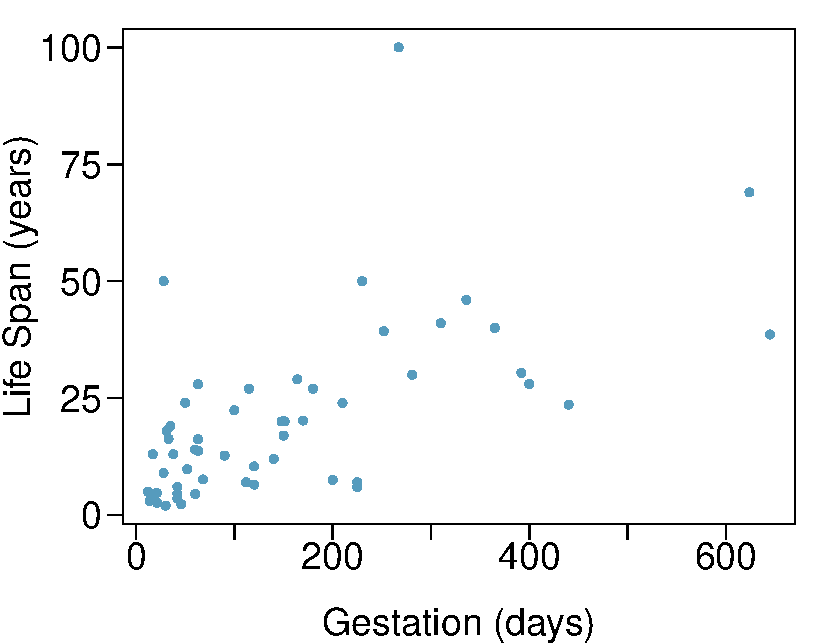
\includegraphics[width = 0.86\textwidth]{ch_summarizing_data/figures/eoce/mammal_life_spans/mammal_life_spans_scatterplot.pdf}
\end{center}
\end{minipage}
}{}

% 2

\eoce{\qt{Associations\label{association_plots}} Indicate which of the plots show a \\[1mm]
\noindent\begin{minipage}[b]{0.35\textwidth}
\begin{parts}
\item positive association
\item negative association
\item no association
\end{parts}
Also determine if the positive and negative associations are linear or nonlinear. Each 
part may refer to more than one plot. \vspace{24mm}
\end{minipage}
\begin{minipage}[b]{0.62\textwidth}
\hfill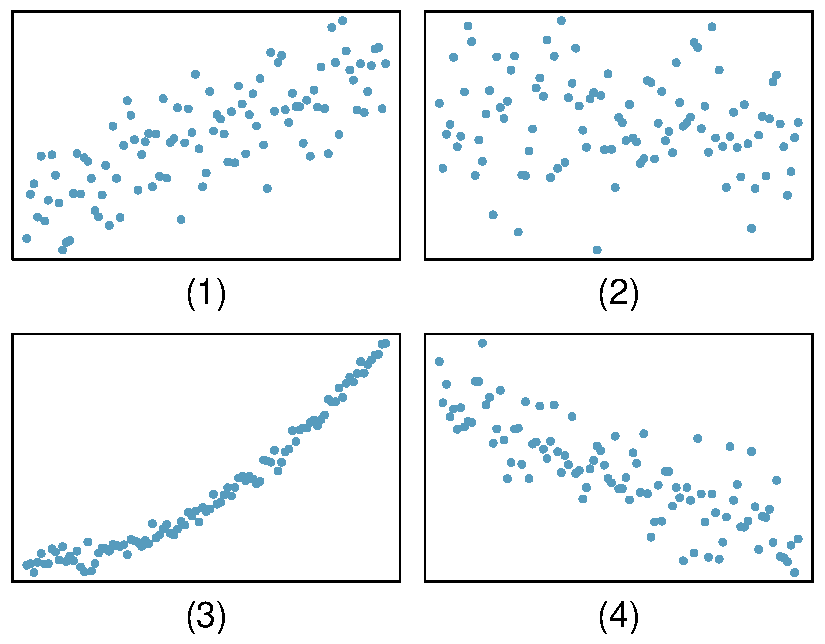
\includegraphics[width = 0.95\textwidth]{ch_summarizing_data/figures/eoce/association_plots/association_plots.pdf}
\end{minipage}
}{}

% 3

\eoce{\qt{Office productivity\label{office_productivity}} Office productivity is relatively low 
when the employees feel no stress about their work or job security. However, high levels 
of stress can also lead to reduced employee productivity. Sketch a plot to represent the 
relationship between stress and productivity.
}{}

% 4

\eoce{\qt{Reproducing bacteria\label{reproducing_bacteria}} Suppose that there is only 
sufficient space and nutrients to support one million bacterial cells in a petri dish. 
You place a few bacterial cells in this petri dish, allow them to reproduce freely, and 
record the number of bacterial cells in the dish over time. Sketch a plot representing 
the relationship between number of bacterial cells and time.
% first exponential
}{}

% 5

\eoce{\qt{Sleeping in college\label{college_sleeping}} A recent article in a college newspaper 
stated that college students get an average of 5.5 hrs of sleep each night. A student who 
was skeptical about this value decided to conduct a survey by randomly sampling 25 
students. On average, the sampled students slept 6.25 hours per night. Identify which 
value represents the sample mean and which value represents the claimed population mean.
}{}

% 6

\eoce{\qt{Parameters and statistics\label{parameters_stats}} Identify which value represents 
the sample mean and which value represents the claimed population mean.
\begin{parts}
\item American households spent an average of about \$52 in 2007 on Halloween 
merchandise such as costumes, decorations and candy. To see if this number had changed, 
researchers conducted a new survey in 2008 before industry numbers were reported. The 
survey included 1,500 households and found that average Halloween spending was \$58 per 
household.
\item The average GPA of students in 2001 at a private university was 3.37. A survey 
on a sample of 203 students from this university yielded an average GPA of 3.59 
a decade later.
\end{parts}
}{}

% 7

\eoce{\qt{Make-up exam\label{makeup_exam}} In a class of 25 students, 24 of them took an exam 
in class and 1 student took a make-up exam the following day. The professor graded the 
first batch of 24 exams and found an average score of 74 points with a standard 
deviation of 8.9 points. The student who took the make-up the following day scored 64 
points on the exam.
\begin{parts}
\item Does the new student's score increase or decrease the average score?
\item What is the new average?
\item Does the new student's score increase or decrease the standard deviation of the 
scores?
\end{parts}
}{}

% 8

\eoce{\qt{Days off at a mining plant\label{days_off_mining}} Workers at a particular mining 
site receive an average of 35 days paid vacation, which is lower than the national 
average. The manager of this plant is under pressure from a local union to increase the 
amount of paid time off. However, he does not want to give more days off to the workers 
because that would be costly. Instead he decides he should fire 10 employees in such a 
way as to raise the average number of days off that are reported by his employees. In 
order to achieve this goal, should he fire employees who have the most number of days 
off, least number of days off, or those who have about the average number of days off?
}{}

% 9

\eoce{\qt{Medians and IQRs} For each part, compare distributions (1) and (2) based on their medians and IQRs. You do not need to calculate these statistics; simply state how the medians and IQRs compare. Make sure to explain your reasoning. 
\begin{multicols}{2}
\begin{parts}
\item (1) 3, 5, 6, 7, 9 \\
(2) 3, 5, 6, 7, 20
\item (1) 3, 5, 6, 7, 9 \\
(2) 3, 5, 7, 8, 9
\item (1) 1, 2, 3, 4, 5 \\
(2) 6, 7, 8, 9, 10
\item (1) 0, 10, 50, 60, 100 \\
(2) 0, 100, 500, 600, 1000
\end{parts}
\end{multicols}
}{}

% 10

\eoce{\qt{Means and SDs} For each part, compare distributions (1) and (2) based on their means and standard deviations. You do not need to calculate these statistics; simply state how the means and the standard deviations compare. Make sure to explain your reasoning. \textit{Hint:} It may be useful to sketch dot plots of the distributions.
\begin{multicols}{2}
\begin{parts}
\item (1) 3, 5, 5, 5, 8, 11, 11, 11, 13 \\
(2) 3, 5, 5, 5, 8, 11, 11, 11, 20 \\
\item (1) -20, 0, 0, 0, 15, 25, 30, 30 \\
(2) -40, 0, 0, 0, 15, 25, 30, 30
\item (1) 0, 2, 4, 6, 8, 10 \\
(2) 20, 22, 24, 26, 28, 30
\item (1) 100, 200, 300, 400, 500 \\
(2) 0, 50, 300, 550, 600
\end{parts}
\end{multicols}
}{}

% 11

\eoce{\qt{Stats scores\label{stats_scores_box}} Below are the final exam scores of twenty 
introductory statistics students.
\begin{center}
57, 66, 69, 71, 72, 73, 74, 77, 78, 78, 79, 79, 81, 81, 82, 83, 83, 88, 89, 94
\end{center}
Create a box plot of the distribution of these scores. The five number summary provided below may be useful.
\begin{center}
\renewcommand\arraystretch{1.5}
\begin{tabular}{ccccc}
Min & Q1    & Q2 (Median)   & Q3    & Max \\
\hline
57  & 72.5  & 78.5          & 82.5  & 94 \\
\end{tabular}
\end{center}
}{}

% 12

\eoce{\qt{Infant mortality\label{infant_mortality}} The infant mortality rate is defined as 
the number of infant deaths per 1,000 live births. This rate is often used as an 
indicator of the level of health in a country. The relative frequency histogram below 
shows the distribution of estimated infant death rates for 224 countries for which such 
data were available in 2014. 
\footfullcite{data:ciaFactbook}

\noindent\begin{minipage}[c]{0.43\textwidth}
\begin{parts}
\item Estimate Q1, the median, and Q3 from the histogram.
\item Would you expect the mean of this data set to be smaller or larger than the 
median? Explain your reasoning.
\end{parts} \vfill \
\end{minipage}
\begin{minipage}[c]{0.52\textwidth}
\hfill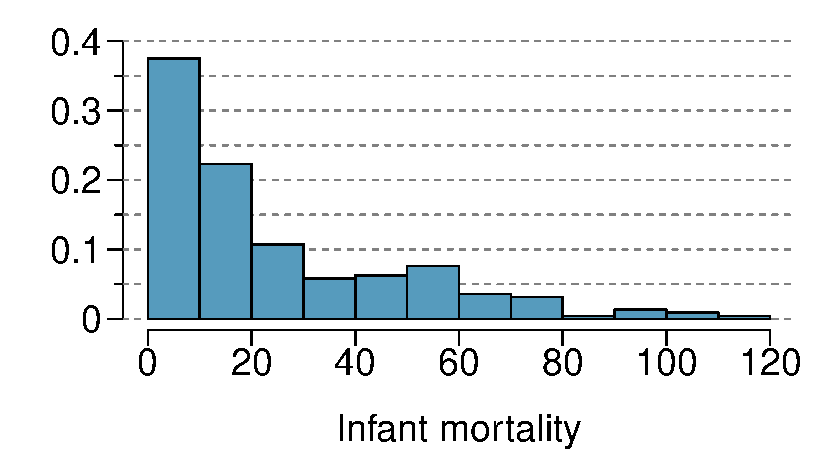
\includegraphics[width = 0.85\textwidth]{ch_summarizing_data/figures/eoce/infant_mortality_rel_freq/infant_mortality_rel_freq_hist.pdf}
\end{minipage}
}{}

% 13

\eoce{\qt{Mix-and-match} Describe the distribution in the histograms below and match them to the box plots. \\
\begin{center}
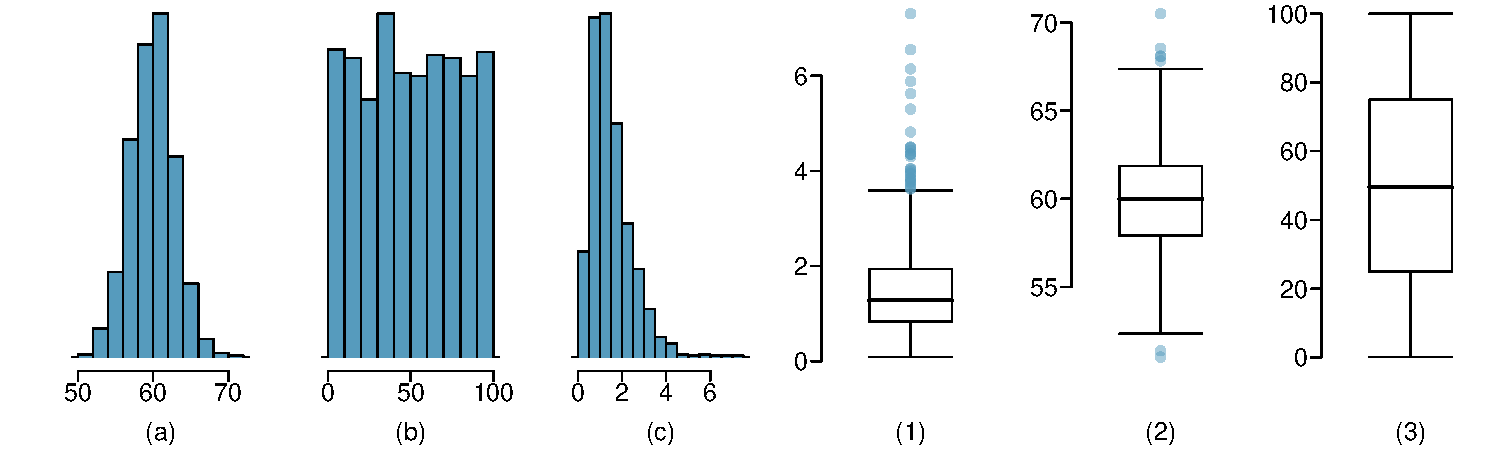
\includegraphics[width=\textwidth]{ch_summarizing_data/figures/eoce/hist_box_match/hist_box_match.pdf}
\end{center}
}{}

% 14

\eoce{\qt{Air quality\label{air_quality_durham}} Daily air quality is measured by the air 
quality index (AQI) reported by the Environmental Protection Agency. This index reports 
the pollution level and what associated health effects might be a concern. The index is 
calculated for five major air pollutants regulated by the Clean Air Act and takes values 
from 0 to 300, where a higher value indicates lower air quality. AQI was reported for a 
sample of 91 days in 2011 in Durham, NC. The relative frequency histogram below shows 
the distribution of the AQI values on these days. \footfullcite{data:durhamAQI:2011}
\begin{minipage}[c]{0.55\textwidth}
\begin{parts}
\item Estimate the median AQI value of this sample.
\item Would you expect the mean AQI value of this sample to be higher or lower than the 
median? Explain your reasoning.
\item Estimate Q1, Q3, and IQR for the distribution.
\item Would any of the days in this sample be considered to have an unusually low or 
high AQI? Explain your reasoning.
\end{parts}
\end{minipage}
\begin{minipage}[c]{0.45\textwidth}
\begin{center}
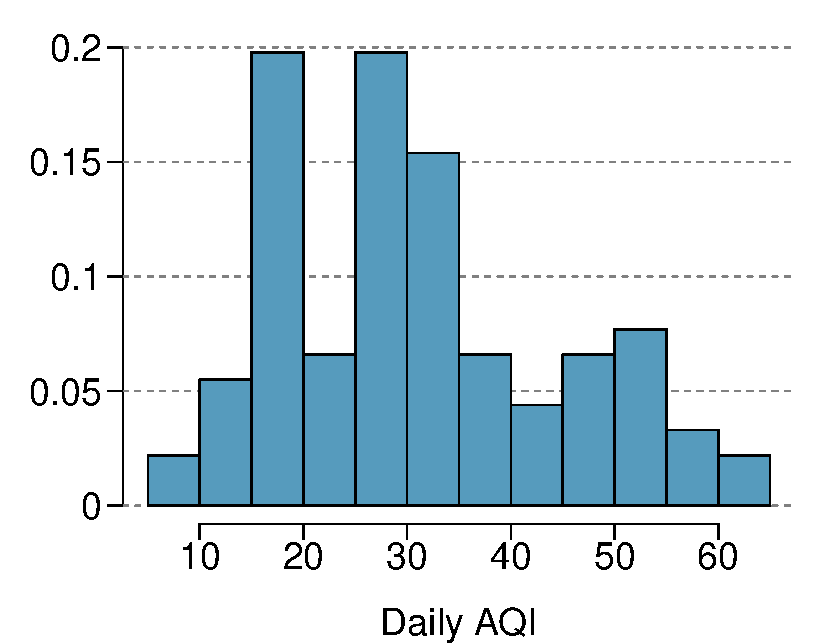
\includegraphics[width = \textwidth]{ch_summarizing_data/figures/eoce/air_quality_durham/air_quality_durham_rel_freq_hist.pdf} 
\end{center}
\end{minipage}
}{}

% 15

\eoce{\qt{Median vs. mean\label{estimate_mean_median_simple}} Estimate the median for the 
400 observations shown in the histogram, and note whether you expect the mean 
to be higher or lower than the median.
\begin{center}
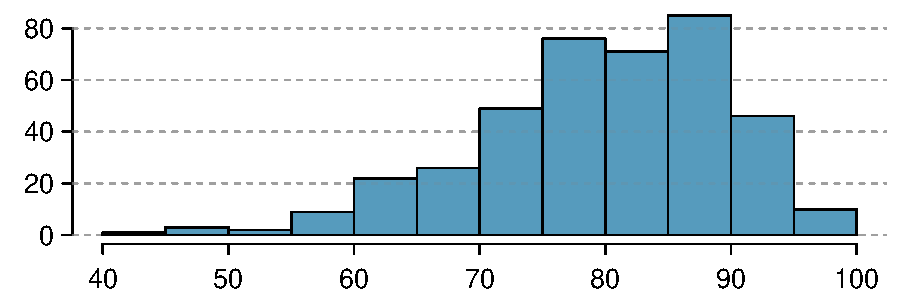
\includegraphics[width = 0.6\textwidth]{ch_summarizing_data/figures/eoce/estimate_mean_median_simple/estimate_mean_median_simple.pdf} 
\end{center}
}{}

% 16

\eoce{\qt{Histograms vs. box plots\label{hist_vs_box}} Compare the two plots below. What 
characteristics of the distribution are apparent in the histogram and not in the box 
plot? What characteristics are apparent in the box plot but not in the histogram?
\begin{center}
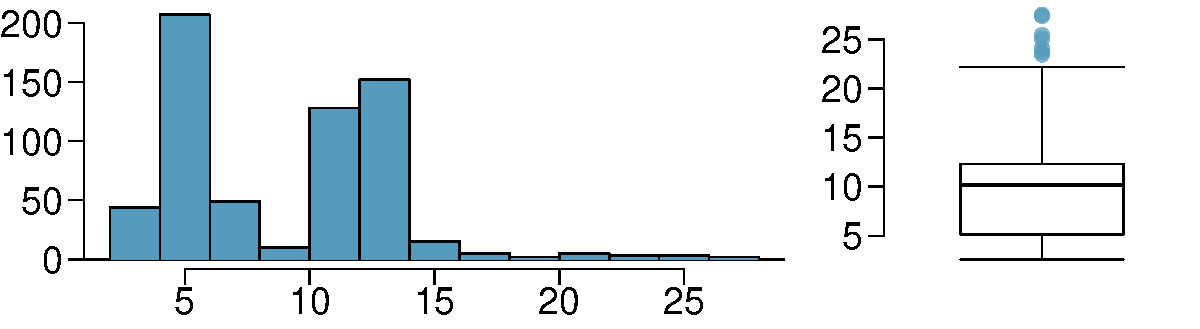
\includegraphics[width = 0.6\textwidth]{ch_summarizing_data/figures/eoce/hist_vs_box/hist_vs_box.pdf}
\end{center}
}{}

% 17

\eoce{\qt{Marathon winners\label{marathon_winners}} The histogram and box plots below show the distribution of finishing times for male and female winners of the New York Marathon between 1970 and 1999.
\begin{center}
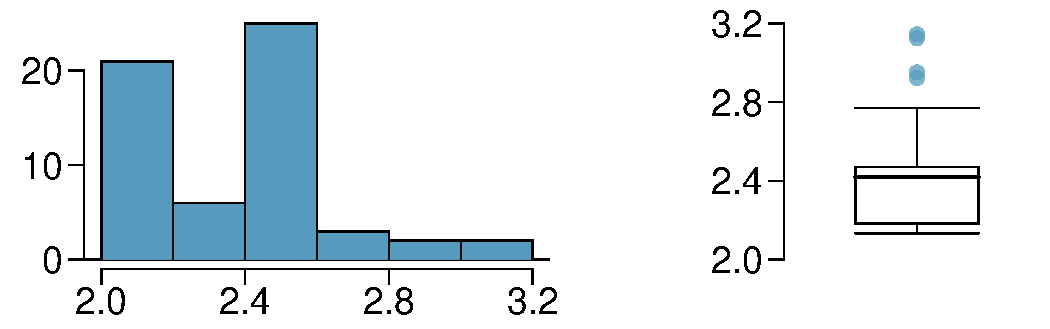
\includegraphics[width=0.56\textwidth]{ch_summarizing_data/figures/eoce/marathon_winners/marathon_winners_hist_box.pdf}
\end{center}
\begin{parts}
\item What features of the distribution are apparent in the histogram and not the box plot? What features are apparent in the box plot but not in the histogram?
\item What may be the reason for the bimodal distribution? Explain.
\item Compare the distribution of marathon times for men and women based on the box plot shown below.
\begin{center}
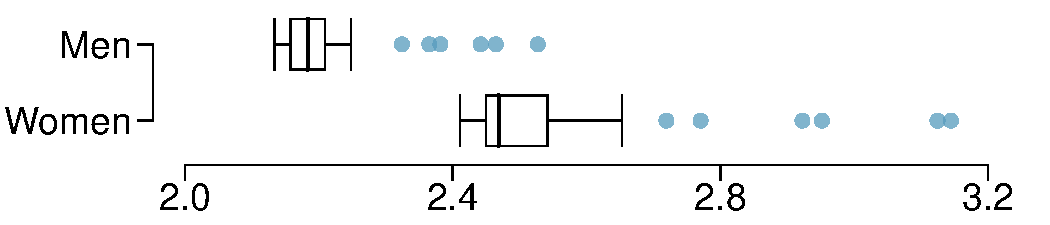
\includegraphics[width=0.56\textwidth]{ch_summarizing_data/figures/eoce/marathon_winners/marathon_winners_gender_box.pdf}
\end{center}
\item The time series plot shown below is another way to look at these data. Describe what is visible in this plot but not in the others.
\end{parts}
\begin{center}
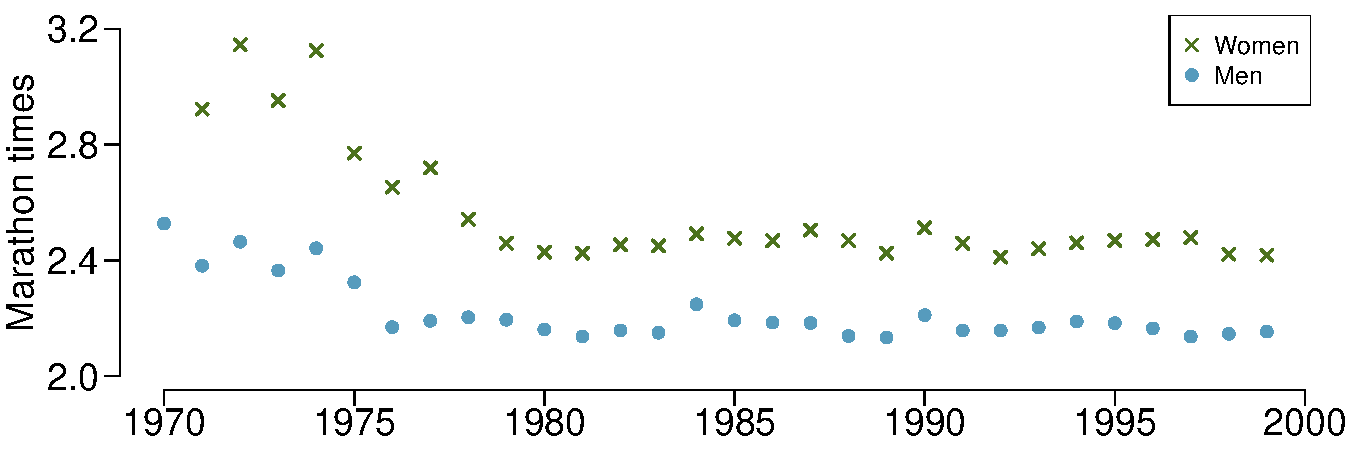
\includegraphics[width=0.6\textwidth]{ch_summarizing_data/figures/eoce/marathon_winners/marathon_winners_time_series.pdf} \\
\end{center}
}{}

% 18

\eoce{\qt{Distributions and appropriate statistics, Part I\label{dist_shape_pets_dist_height}} 
For each of the following, state whether you expect the distribution to be 
symmetric, right skewed, or left skewed. Also specify whether the mean or 
median would best represent a typical observation in the data, and whether 
the variability of observations would be best represented using the 
standard deviation or IQR. Explain your reasoning.
\begin{parts}
\item Number of pets per household. 
\item Distance to work, i.e. number of miles between work and home.
\item Heights of adult males.
\end{parts}
}{}

% 19

\eoce{\qt{Distributions and appropriate statistics, Part II\label{dist_shape_housing_alcohol_salary}} 
For each of the following, state whether you expect the distribution to be symmetric, 
right skewed, or left skewed. Also specify whether the mean or median would best 
represent a typical observation in the data, and whether the variability of observations 
would be best represented using the standard deviation or IQR. Explain your reasoning.
\begin{parts}
\item Housing prices in a country where 25\% of the houses cost below \$350,000, 
50\% of the houses cost below \$450,000, 75\% of the houses cost below \$1,000,000 
and there are a meaningful number of houses that cost more than \$6,000,000.
\item Housing prices in a country where 25\% of the houses cost below \$300,000, 
50\% of the houses cost below \$600,000, 75\% of the houses cost below \$900,000 
and very few houses that cost more than \$1,200,000.
\item Number of alcoholic drinks consumed by college students in a given week. 
Assume that most of these students don't drink since they are under 21 years old, 
and only a few drink excessively.
\item Annual salaries of the employees at a Fortune 500 company where only a few 
high level executives earn much higher salaries than all the other employees.
\end{parts}
}{}

% 20

\eoce{\qt{TV watchers\label{dist_shape_TV_watchers}} Students in an AP Statistics class 
were asked how many hours of television they watch per week (including online 
streaming). This sample yielded an average of 4.71 hours, with a standard 
deviation of 4.18 hours. Is the distribution of number of hours students watch 
television weekly symmetric? If not, what shape would you expect this distribution 
to have? Explain your reasoning.
}{}

% 21

\eoce{\qt{Exam scores\label{dist_shape_exam_scores}} The average on a history exam 
(scored out of 100 points) was 85, with a standard deviation of 15. Is the 
distribution of the scores on this exam symmetric? If not, what shape would 
you expect this distribution to have? Explain your reasoning.
}{}

% 22

\eoce{\qt{Facebook friends\label{dist_shape_fb_friends}} Facebook data indicate that 
50\% of Facebook users have 100 or more friends, and that the average friend 
count of users is 190. What do these findings suggest about the shape of the 
distribution of number of friends of Facebook users? \footfullcite{Backstrom:2011}
}{}

% 23

\eoce{\qt{A new statistic\label{new_stat}} The statistic $\frac{\bar{x}}{median}$ can 
be used as a measure of skewness. Suppose we have a distribution where all 
observations are greater than 0, $x_i > 0$. What is the expected shape of 
the distribution under the following conditions? Explain your reasoning.
\begin{parts}
\item $\frac{\bar{x}}{median} = 1$
\item $\frac{\bar{x}}{median} < 1$
\item $\frac{\bar{x}}{median} > 1$
\end{parts}
}{}

% 24

\eoce{\qt{Income at the coffee shop\label{income_coffee_shop}} The first histogram 
below shows the distribution of the yearly incomes of 40 patrons at a college 
coffee shop. Suppose two new people walk into the coffee shop: one making 
\$225,000 and the other \$250,000. The second histogram shows the new income 
distribution. Summary statistics are also provided. \\
\begin{minipage}[c]{0.57\textwidth}
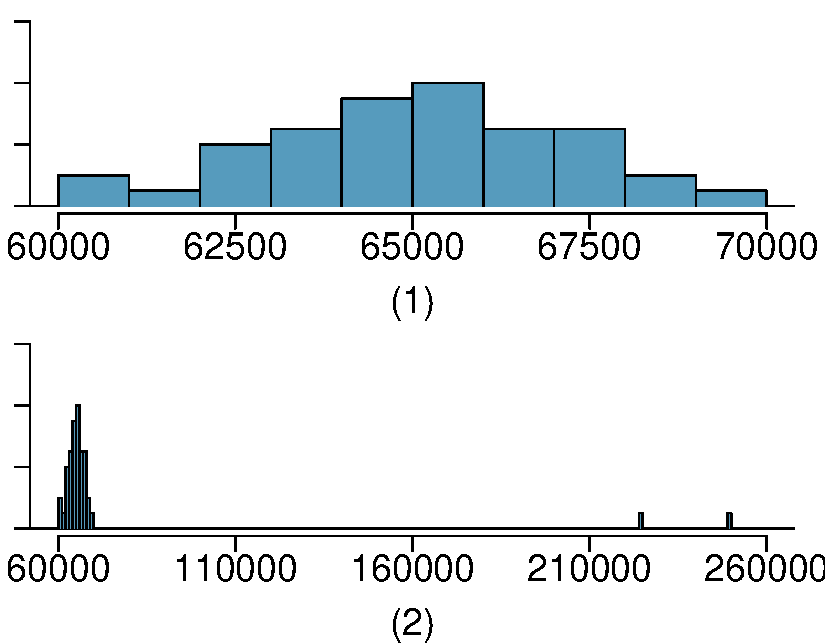
\includegraphics[width=\textwidth]{ch_summarizing_data/figures/eoce/income_coffee_shop/income_coffee_shop.pdf}
\end{minipage}
\begin{minipage}[c]{0.4\textwidth}
\begin{center}
\begin{tabular}{rrr}
\hline
        & (1)       & (2) \\ 
\hline
n       & 40        & 42 \\ 
Min.    & 60,680    & 60,680 \\ 
1st Qu. & 63,620    & 63,710 \\ 
Median  & 65,240    & 65,350 \\ 
Mean    & 65,090    & 73,300 \\ 
3rd Qu. & 66,160    & 66,540 \\ 
Max.    & 69,890    & 250,000 \\ 
SD      & 2,122     & 37,321 \\ 
\hline
\end{tabular}
\end{center}
\end{minipage}
\begin{parts}
\item Would the mean or the median best represent what we might think of as a 
typical income for the 42 patrons at this coffee shop? What does this say about 
the robustness of the two measures?
\item Would the standard deviation or the IQR best represent the amount of 
variability in the incomes of the 42 patrons at this coffee shop? What does 
this say about the robustness of the two measures?
\end{parts}
}{}

% 25

\eoce{\qt{Midrange\label{midrange}} The \textit{midrange} of a distribution is defined as 
the average of the maximum and the minimum of that distribution. Is this statistic 
robust to outliers and extreme skew? Explain your reasoning
}{}

% 26

\eoce{\qt{Commute times\label{county_commute_times}} The US census collects data on 
time it takes Americans to commute to work, among many other variables. The 
histogram below shows the distribution of average commute times in 3,142 US 
counties in 2010. Also shown below is a spatial intensity map of the same data.
\begin{center}
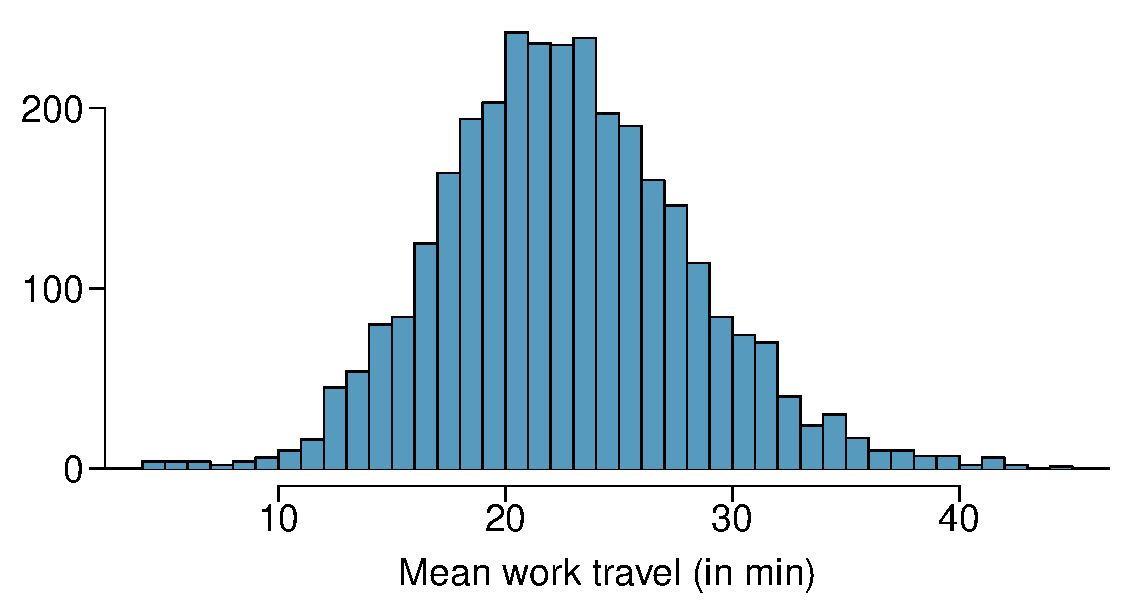
\includegraphics[width=0.48\textwidth]{ch_summarizing_data/figures/eoce/county_commute_times/county_commute_times_hist.pdf}
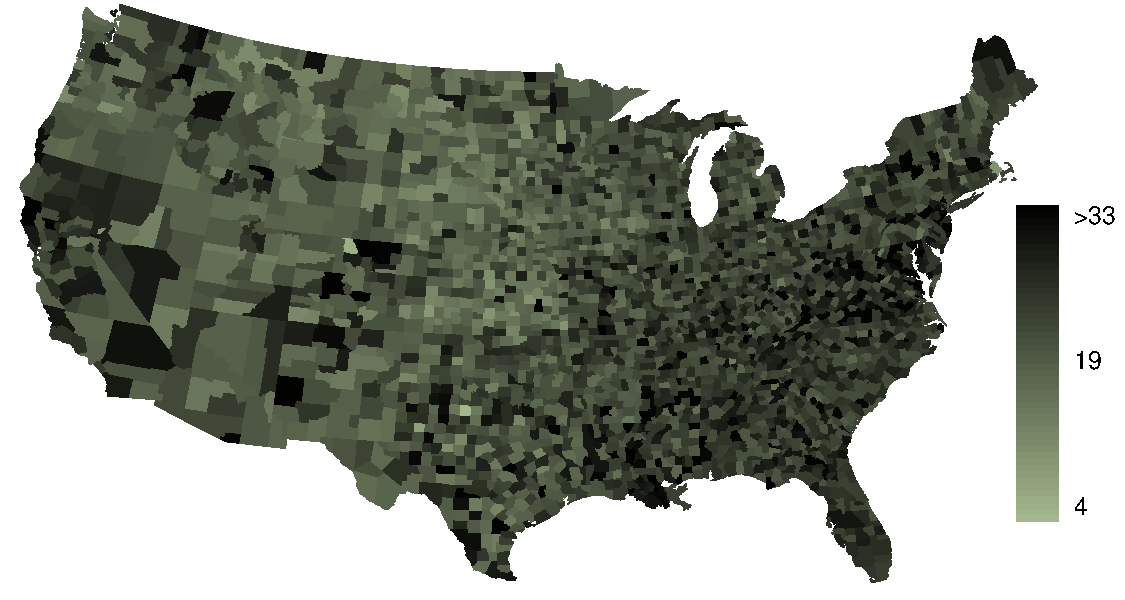
\includegraphics[width=0.48\textwidth]{ch_summarizing_data/figures/eoce/county_commute_times/county_commute_times_map.pdf}
\end{center}
\begin{parts}
\item Describe the numerical distribution and comment on whether or not a log 
transformation may be advisable for these data.
\item Describe the spatial distribution of commuting times using the map below.
\end{parts} 
}{}

% 27

\eoce{\qt{Hispanic population\label{county_hispanic_pop}} The US census collects 
data on race and ethnicity of Americans, among many other variables. The 
histogram below shows the distribution of the percentage of the population 
that is Hispanic in 3,142 counties in the US in 2010. Also shown is a 
histogram of logs of these values.
\begin{center}
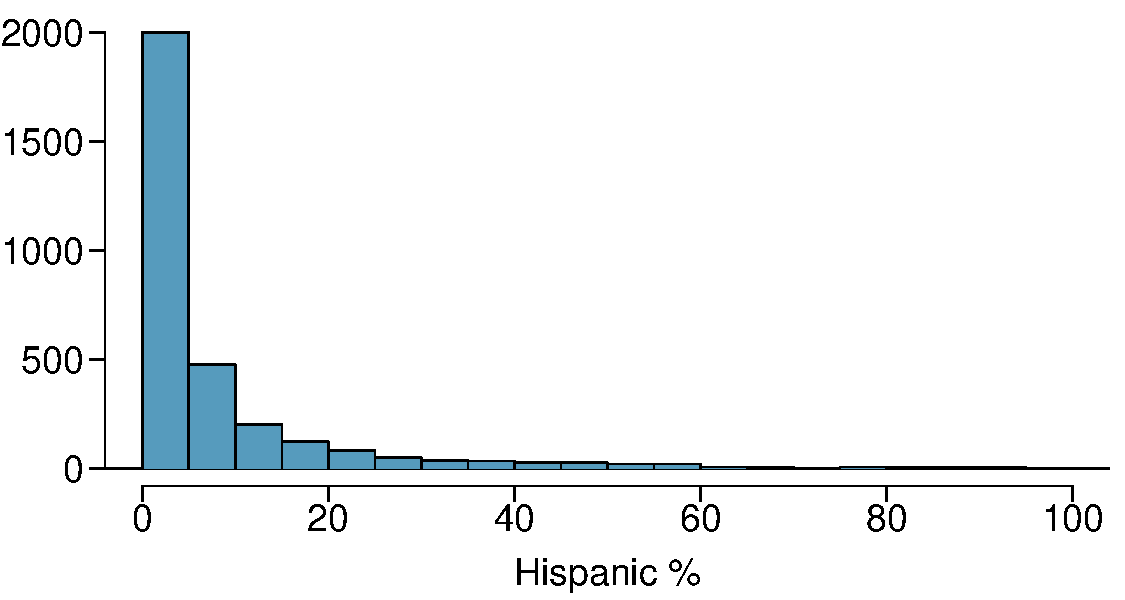
\includegraphics[width=0.48\textwidth]{ch_summarizing_data/figures/eoce/county_hispanic_pop/county_hispanic_pop_hist.pdf}
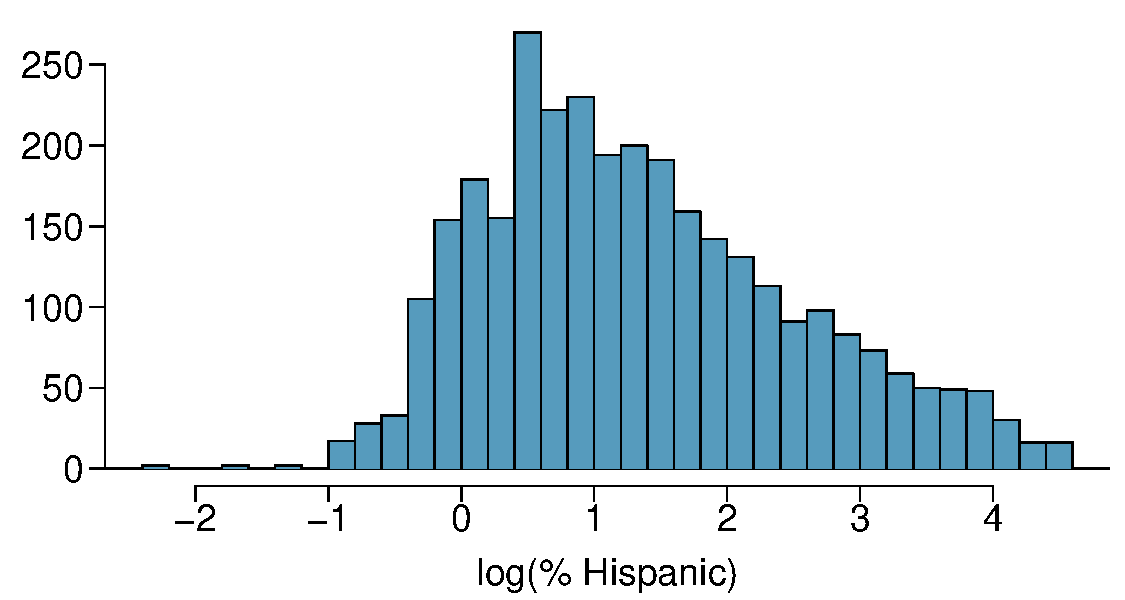
\includegraphics[width=0.48\textwidth]{ch_summarizing_data/figures/eoce/county_hispanic_pop/county_hispanic_pop_log_hist.pdf}
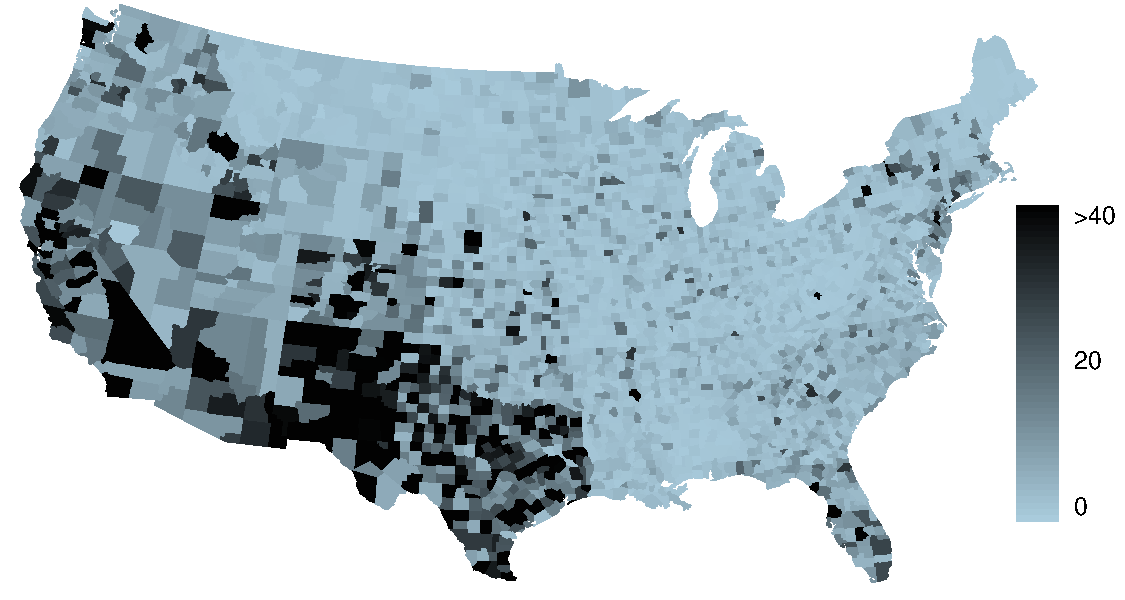
\includegraphics[width=0.48\textwidth]{ch_summarizing_data/figures/eoce/county_hispanic_pop/county_hispanic_pop_map.pdf}
\end{center}
\begin{parts}
\item Describe the numerical distribution and comment on why we might want 
to use log-transformed values in analyzing or modeling these data.
\item What features of the distribution of the Hispanic population in US 
counties are apparent in the map but not in the histogram? What features are 
apparent in the histogram but not the map?
\item Is one visualization more appropriate or helpful than the other? Explain 
your reasoning.
\end{parts} 
}{}
}




\section{Considering categorical data}
\label{categoricalData}

\index{data!loans|(}

In this section, we will introduce tables and other basic tools
for categorical data that are used throughout this book.
The \data{loan50} data set represents a sample from a larger
loan data set called \data{loans}.
This larger data set contains information on 10,000 loans made
through Lending Club.
We~will examine the relationship between
\var{homeownership}, which for the \data{loans} data can take
a value of \resp{rent}, \resp{mortgage}
(owns but has a mortgage), or \resp{own},
and \var{app\us{}type},
which indicates whether the loan application was made
with a partner or whether it was an individual application.
% library(openintro); dim(loans_full_schema)


\subsection{Contingency tables and bar plots}

\newcommand{\loanapphomeAA}{3496}
\newcommand{\loanapphomeAB}{3839}
\newcommand{\loanapphomeAC}{1170}
\newcommand{\loanapphomeAD}{8505}
\newcommand{\loanapphomeBA}{362}
\newcommand{\loanapphomeBB}{950}
\newcommand{\loanapphomeBC}{183}
\newcommand{\loanapphomeBD}{1495}
\newcommand{\loanapphomeDA}{3858}
\newcommand{\loanapphomeDAPt}{0.3858} % Overall frequency
\newcommand{\loanapphomeDB}{4789}
\newcommand{\loanapphomeDC}{1353}
\newcommand{\loanapphomeDD}{10000}
\newcommand{\loanapphomeN}{\loanapphomeDD{}}

Figure~\ref{loan_home_app_type_totals} summarizes two variables:
\var{app\us{}type}
%\footnote{For those readers already familiar
%  with \emph{joint probabilities}, \resp{joint} in the table
%  refers to a level of the \var{app\us{}type} variable
%  for a joint application.
%  The does not refer to a joint probability!}
and \var{homeownership}.
A table that summarizes data for two categorical variables in
this way is called a \term{contingency table}.
Each value in the table represents the number of times
a particular combination of variable outcomes occurred.
For example, the value \loanapphomeAA{} corresponds to the number of
loans in the data set where the borrower rents their home
and the application type was by an individual.
Row and column totals are also included.
The \term{row totals} \index{contingency table!row totals}
provide the total counts across each row
(e.g. $\loanapphomeAA{} + \loanapphomeAB{} +
  \loanapphomeAC{} = \loanapphomeAD{}$),
and \term{column totals} \index{contingency table!column totals}
are total counts down each column.
We can also create a table that shows only the overall 
percentages or proportions for each combination of categories,
or we can create a table for a single variable,
such as the one shown in Figure~\ref{loan_homeownership_totals}
for the \var{homeownership} variable.

\begin{figure}[ht]
\centering
\begin{tabular}{ll  ccc  rr}
  & & \multicolumn{3}{c}{\bf \var{homeownership}} & \\
  \cline{3-5}
  & & rent & mortgage & own & Total & \hspace{2mm}\  \\ 
  \cline{2-6}
  & individual &
      \loanapphomeAA{} &
      \loanapphomeAB{} &
      \loanapphomeAC{} &
      \loanapphomeAD{} \\
  \raisebox{1.5ex}[0pt]{\var{app\us{}type}} &
  joint &
      \loanapphomeBA{} &
      \loanapphomeBB{} &
	  \loanapphomeBC{} &
	  \loanapphomeBD{} \\
  \cline{2-6}
  & Total &
      \loanapphomeDA{} &
      \loanapphomeDB{} &
      \loanapphomeDC{} &
      \loanapphomeDD{} \\
  \cline{2-6}
\end{tabular}
\caption{A contingency table for
    \var{app\us{}type} and \var{homeownership}.}
\label{loan_home_app_type_totals}
%library(openintro); library(xtable); tab <- table(loans_full_schema[,c("application_type", "homeownership")])[, c("RENT", "MORTGAGE", "OWN")]; xtable(tab); rowSums(tab); colSums(tab); sum(tab)
\end{figure}

\begin{figure}[htb]
\centering
\begin{tabular}{lc}
  \hline
  \var{homeownership} & Count \\
  \hline
  rent & \loanapphomeDA{} \\
  mortgage & \loanapphomeDB{} \\
  own & \loanapphomeDC{} \\
  \hline
  Total & \loanapphomeDD{} \\ 
  \hline
\end{tabular}
\caption{A table summarizing the frequencies of each
    value for the \var{homeownership} variable.}
\label{loan_homeownership_totals}
\end{figure}

A bar plot is a common way to display a single
categorical variable.
The left panel of Figure~\ref{loan_homeownership_bar_plot}
shows a \term{bar plot} for the \var{homeownership} variable.
In the right panel, the counts are converted into proportions,
showing the proportion of observations that are in each level
(e.g. $\loanapphomeDA{} / \loanapphomeDD{} = 0.3858$ for
  \resp{rent}).

\begin{figure}[bht]
  \centering
  \Figure{0.82}{loan_homeownership_bar_plot}
  \caption{Two bar plots of \var{number}.
      The left panel shows the counts, and the right panel
      shows the proportions in each group.}
  \label{loan_homeownership_bar_plot}
\end{figure}


\subsection{Row and column proportions}

Sometimes it is useful to understand the fractional breakdown
of one variable in another,
and we can modify our contingency table to provide such a view.
Figure~\ref{rowPropAppTypeHomeownership}
shows the
\termsub{row proportions}{contingency table!row proportions}
for Figure~\ref{loan_home_app_type_totals},
which are computed as the counts divided by their row totals.
The value \loanapphomeAA{} at the intersection of
\resp{individual} and \resp{rent} is replaced by
$\loanapphomeAA{}/\loanapphomeAD{} = 0.411$,
i.e. \loanapphomeAA{} divided by its row total,
\loanapphomeAD{}.
So what does 0.411 represent?
It corresponds to the proportion of individual
applicants who rent.

\begin{figure}
\centering
\begin{tabular}{l rrr r}
  \hline
  & rent & mortgage & own & Total \\
  \hline
  individual & 
%      $\loanapphomeAA{}/\loanapphomeAD{} = 0.411$ &
%      $\loanapphomeAB{}/\loanapphomeAD{} = 0.451$ &
%      $\loanapphomeAC{}/\loanapphomeAD{} = 0.138$ &
      0.411 &
      0.451 &
      0.138 &
      1.000 \\
  joint &
%      $\loanapphomeBA{}/\loanapphomeBD{} = 0.242$ &
%      $\loanapphomeBB{}/\loanapphomeBD{} = 0.635$ &
%      $\loanapphomeBC{}/\loanapphomeBD{} = 0.122$ &
      0.242 &
      0.635 &
      0.122 &
      1.000 \\
  \hline
  Total &
%      $\loanapphomeDA{}/\loanapphomeDD{} = 0.386$ &
%      $\loanapphomeDB{}/\loanapphomeDD{} = 0.479$ &
%      $\loanapphomeDC{}/\loanapphomeDD{} = 0.135$ &
      0.386 &
      0.479 &
      0.135 &
      1.000 \\
  \hline
\end{tabular}
\caption{A contingency table with row proportions
    for the \var{app\us{}type} and
    \var{homeownership} variables.
    The row total is off by 0.001 for the
    \resp{joint} row due to a rounding error.}
\label{rowPropAppTypeHomeownership}
\end{figure}

A contingency table of the column proportions is computed in a similar way, where each \termsub{column proportion}{contingency table!column proportion} is computed as the count divided by the corresponding column total. Figure~\ref{colPropAppTypeHomeownership} shows such a table, and here the value 0.906 indicates that 90.6\% of renters applied as individuals for the loan. This rate is higher compared to loans from people with mortgages (80.2\%) or who own their home (85.1\%). Because these rates vary between the three levels of \var{homeownership} (\resp{rent}, \resp{mortgage}, \resp{own}), this provides evidence that the \var{app\us{}type} and \var{homeownership} variables are associated.

\begin{figure}[h]
\centering%\small
\begin{tabular}{l rrr r}
  \hline
  & rent & mortgage & own & Total \\
  \hline
  individual &
%      $\loanapphomeAA{}/\loanapphomeDA{} = 0.906$ &
%      $\loanapphomeAB{}/\loanapphomeDB{} = 0.802$ &
%      $\loanapphomeAC{}/\loanapphomeDC{} = 0.865$ &
%      $\loanapphomeAD{}/\loanapphomeDD{} = 0.851$ \\
      0.906 &
      0.802 &
      0.865 &
      0.851 \\
  joint &
%      $\loanapphomeBA{}/\loanapphomeDA{} = 0.094$ &
%      $\loanapphomeBB{}/\loanapphomeDB{} = 0.198$ &
%      $\loanapphomeBC{}/\loanapphomeDC{} = 0.135$ &
%      $\loanapphomeBD{}/\loanapphomeDD{} = 0.150$ \\
      0.094 &
      0.198 &
      0.135 &
      0.150 \\
  \hline
  Total & 1.000 & 1.000 & 1.000 & 1.000 \\
  \hline
\end{tabular}
\caption{A contingency table with column proportions for the
    \var{app\us{}type} and \var{homeownership}
    variables.
    The total for the last column is off by 0.001 due
    to a rounding error.}
\label{colPropAppTypeHomeownership}
\end{figure}

We could also have checked for an association between \var{app\us{}type} and \var{homeownership} in Figure~\ref{rowPropAppTypeHomeownership} using row proportions. When comparing these row proportions, we would look down columns to see if the fraction of loans where the borrower rents, has a mortgage, or owns varied across the \resp{individual} to \resp{joint} application types.

\begin{exercisewrap}
\begin{nexercise}
(a)~What does 0.451 represent in
Figure~\ref{rowPropAppTypeHomeownership}?

(b)~What does 0.802 represent in
Figure~\ref{colPropAppTypeHomeownership}?\footnotemark{}
\end{nexercise}
\end{exercisewrap}
\footnotetext{(a)~0.451 represents the proportion of individual
  applicants who have a mortgage.
  (b)~0.802 represents the fraction
  of applicants with mortgages who applied as individuals.}

\begin{exercisewrap}
\begin{nexercise}
(a)~What does 0.122 at the intersection of \resp{joint} and
\resp{own} represent in
Figure~\ref{rowPropAppTypeHomeownership}?

(b)~What does 0.135 represent in the
Figure~\ref{colPropAppTypeHomeownership}?\footnotemark{}
\end{nexercise}
\end{exercisewrap}
\footnotetext{(a)~0.122 represents the fraction of joint borrowers
  who own their home.
  (b)~0.135 represents the home-owning borrowers
  who had a joint application for the loan.}

\begin{examplewrap}
\begin{nexample}{
    Data scientists use statistics to filter spam from incoming
    email messages.
    By noting specific characteristics of an email,
    a data scientist may be able to classify some emails as spam
    or not spam with high accuracy.
    One such characteristic is whether the email
    contains no numbers, small numbers, or big numbers.
    Another characteristic is the email format, which
    indicates whether or not an email has any HTML content,
    such as bolded text.
    We'll focus on email format and spam status using the
    \data{email} data set, and these variables are summarized
    in a contingency table in
    Figure~\ref{emailSpamHTMLTableTotals}.
    Which would be more helpful to someone hoping to classify
    email as spam or regular email for this table:
    row or column proportions?}
  \label{weighingRowColumnProportions}
  A data scientist would be interested in how the proportion
  of spam changes within each email format.
  This corresponds to column proportions:
  the proportion of spam in plain text emails
  and the proportion of spam in HTML emails.

  If we generate the column proportions, we can see
  that a higher fraction of plain text emails are
  spam ($209/1195 = 17.5\%$)
  than compared to HTML emails ($158/2726 = 5.8\%$).
  This information on its own is insufficient to classify
  an email as spam or not spam, as over 80\% of plain text
  emails are not spam.
  Yet, when we carefully combine this information with many
  other characteristics,
  we stand a reasonable chance of being able to classify
  some emails as spam or not spam with confidence.
\end{nexample}
\end{examplewrap}

\begin{figure}[ht]
\centering
\begin{tabular}{l cc r}
  \hline
  & text & HTML & Total \\ 
  \hline
  spam & 209 & 158 & 367 \\ 
  not spam & 986 & 2568 & 3554 \\ 
  \hline
  Total & 1195 & 2726 & 3921 \\
  \hline
\end{tabular}
\caption{A contingency table for \var{spam} and \var{format}.}
\label{emailSpamHTMLTableTotals}
%library(openintro); library(xtable); data(email); tab <- table(email[,c("spam", "format")])[2:1,]; tab; colSums(tab); rowSums(tab)
\end{figure}

Example~\ref{weighingRowColumnProportions} points out
that row and column proportions are not equivalent.
Before settling on one form for a table,
it is important to consider each to ensure that the
most useful table is constructed.
However, sometimes it simply isn't clear which, if either,
is more useful.

\begin{examplewrap}
\begin{nexample}{Look back to
    Tables~\ref{rowPropAppTypeHomeownership}
    and~\ref{colPropAppTypeHomeownership}.
    Are there any obvious scenarios where one might be more
    useful than the other?}
  None that we thought were obvious!
  What is distinct about \var{app\us{}type}
  and \var{homeownership} vs the email example is that
  these two variables don't have a clear explanatory-response
  variable relationship that we might hypothesize
  (see Section~\ref{explanatoryAndResponse} for these terms).
  Usually it is most useful to ``condition'' on the
  explanatory variable.
  For instance, in the email example, the email format
  was seen as a possible explanatory variable of whether
  the message was spam, so we would find it more interesting
  to compute the relative frequencies (proportions)
  for each email format.
\end{nexample}
\end{examplewrap}

%\Comment{Any risk with the above example that students
%  would think they need not know how to describe (what
%  are effectively) conditional probabilities based
%  on row or column proportions?
%  If so, we could add in an exercise that calls this
%  out and requires them to create such a description.}


\subsection{Using a bar plot with two variables}
\label{bar_plots_subsection}

Contingency tables using row or column proportions
are especially useful for examining how two categorical
variables are related.
Stacked bar plots provide a way to visualize
the information in these tables.

A \termsub{stacked bar plot}{bar plot!stacked bar plot}
\index{bar plot!segmented bar plot}
is a graphical display of contingency table information.
For example, a~stacked bar plot representing
Figure~\ref{colPropAppTypeHomeownership}
is shown in Figure~\ref{loan_app_type_home_seg_bar},
where we have first created a bar plot using the
\var{homeownership} variable and then divided each group
by the levels of \mbox{\var{app\us{}type}}.

One related visualization to the stacked bar plot is the
\termsub{side-by-side bar plot}{bar plot!side-by-side},
where an example is shown in
Figure~\ref{loan_app_type_home_sbs_bar}.

For the last type of bar plot we introduce,
the column proportions for the
\var{app\us{}type} and \var{homeownership} contingency table
have been translated into a standardized stacked bar plot
in Figure~\ref{loan_app_type_home_seg_bar_standardized}.
This type of visualization is helpful in understanding
the fraction of individual or joint loan applications
for borrowers in each level of \var{homeownership}.
Additionally, since the proportions of \resp{joint}
and \resp{individual} vary across the groups,
we can conclude that the two variables are associated.

\newcommand{\loanapptypehomesegbarplotwidth}{0.46\textwidth}
\begin{figure}[h]
  \centering
  \subfigure[]{
    \Figuress{\loanapptypehomesegbarplotwidth}
        {loan_app_type_home_seg_bar}
        {loan_app_type_home_seg_bar}
    \label{loan_app_type_home_seg_bar}
  }
  \subfigure[]{
    \Figuress{\loanapptypehomesegbarplotwidth}
        {loan_app_type_home_seg_bar}
        {loan_app_type_home_sbs_bar}
    \label{loan_app_type_home_sbs_bar}
  }
  \subfigure[]{
    \Figuress{\loanapptypehomesegbarplotwidth}
        {loan_app_type_home_seg_bar}
        {loan_app_type_home_seg_bar_standardized}
    \label{loan_app_type_home_seg_bar_standardized}
  }
%  \subtable{
%    \footnotesize
%    \begin{tabular}{l  ccc  r}
%      \multicolumn{5}{l}{Contingency table summarizing}\\
%      \multicolumn{5}{l}{application type and homeownership:} \\
%      \\
%      & \multicolumn{3}{c}{\bf \var{homeownership}} & \\
%      \cline{2-4}
%      \var{app\us{}type} &
%          rent & mortgage & own & Total \\ 
%      \hline
%      individual &
%          \loanapphomeAA{} &
%          \loanapphomeAB{} &
%          \loanapphomeAC{} &
%          \loanapphomeAD{} \\
%      joint &
%          \loanapphomeBA{} &
%          \loanapphomeBB{} &
%    	  \loanapphomeBC{} &
%    	  \loanapphomeBD{} \\
%      \hline
%      Total &
%          \loanapphomeDA{} &
%          \loanapphomeDB{} &
%          \loanapphomeDC{} &
%          \loanapphomeDD{} \\
%      \hline
%      \ \\
%      \ \\
%      \multicolumn{5}{l}{Version of the table}\\
%      \multicolumn{5}{l}{with column proportions:} \\
%      \\
%      & \multicolumn{3}{c}{\bf \var{homeownership}} & \\
%      \cline{2-4}
%      \var{app\us{}type} &
%          rent & mortgage & own & Total \\ 
%      \hline
%      individual &
%          0.906 &
%          0.802 &
%          0.865 &
%          0.851 \\
%      joint &
%          0.094 &
%          0.198 &
%          0.135 &
%          0.150 \\
%      \hline
%      Total & 1.000 & 1.000 & 1.000 & 1.000 \\
%      \hline
%      \ \\
%    \end{tabular}
%    \label{loan_app_type_home_copied_table}
%  }
  \caption{\subref{loan_app_type_home_seg_bar} Stacked
      bar plot for \var{homeownership},
      where the counts have been further broken down
      by \var{app\us{}type}.
      \subref{loan_app_type_home_sbs_bar}~Side-by-side
      bar plot for \var{homeownership}
      and \var{app\us{}type}.
      \subref{loan_app_type_home_seg_bar_standardized}~Standardized
      version of the stacked bar plot.
      \subref{loan_app_type_home_copied_table}~A
      contingency table for
      \var{app\us{}type} and \var{homeownership}.}
  \label{loan_app_type_home_seg_bar_plot}
\end{figure}

\begin{examplewrap}
\begin{nexample}{Examine the three bar plots in
    Figure~\ref{loan_app_type_home_seg_bar_plot}.
    When is the stacked, side-by-side, or standardized
    stacked bar plot the most useful?}
  The stacked bar plot is most useful when it's reasonable
  to assign one variable as the explanatory variable and
  the other variable as the response, since we are effectively
  grouping by one variable first and then breaking it down by
  the others.

  Side-by-side bar plots are more agnostic in their display
  about which variable, if any, represents the explanatory
  and which the response variable.
  It is also easy to discern the number of cases
  in of the six different group combinations.
  However, one downside
  is that it tends to require more horizontal space;
  the narrowness of Figure~\ref{loan_app_type_home_sbs_bar}
  makes the plot feel a bit cramped.
  Additionally, when two groups are of very different sizes,
  as we see in the \resp{own} group relative to either of the
  other two groups,
  it is difficult to discern if there is an association
  between the variables.

  The standardized stacked bar plot is helpful if the primary
  variable in the stacked bar plot is relatively imbalanced,
  e.g. the \resp{own} category has only a third of the
  observations in the \resp{mortgage} category,
  making the simple stacked bar plot less useful for
  checking for an association.
  The major downside of the standardized version
  is that we lose all sense of how many cases each of the
  bars represents.
\end{nexample}
\end{examplewrap}

%Before settling on a particular bar plot, consider each
%carefully.
%It can also be useful to make a couple of the versions,
%which will offer different views and insights into the data
%than if only one bar plot variant is reviewed.

\subsection{Mosaic plots}
\label{mosaic_plots_subsection}

A \term{mosaic plot} is a visualization technique
suitable for contingency tables that resembles
a standardized stacked bar plot with the benefit
that we still see the relative group sizes of the
primary variable as well.

To get started in creating our first mosaic plot,
we'll break a square into columns for each category
of the \var{homeownership} variable,
with the result shown in Figure~\ref{loan_home_mosaic}.
Each column represents a level of \var{homeownership},
and the column widths correspond to the proportion of
loans in each of those categories.
For~instance, there are fewer loans where the borrower
is an owner than where the borrower has a mortgage.
In general, mosaic plots use box \emph{areas}
to represent the number of cases in each category.

\begin{figure}[h]
  \centering
  \subfigure[]{
    \Figures{0.36}
        {loan_app_type_home_mosaic_plot}
        {loan_home_mosaic}
    \label{loan_home_mosaic}
  }
  \subfigure[]{
    \Figures{0.44}
        {loan_app_type_home_mosaic_plot}
        {loan_app_type_home_mosaic}
    \label{loan_app_type_home_mosaic}
  }
  \caption{\subref{loan_home_mosaic}~The one-variable mosaic
      plot for \var{homeownership}.
      \subref{loan_app_type_home_mosaic}~Two-variable mosaic
      plot for both \var{homeownership}
      and \var{app\us{}type}.}
  \label{loan_app_type_home_mosaic_plot}
\end{figure}

To create a completed mosaic plot, the single-variable
mosaic plot is further divided into pieces in
Figure~\ref{loan_app_type_home_mosaic} using the
\var{app\us{}type} variable.
Each column is split proportional to the
number of loans from individual and joint
borrowers.
For example, the second column represents loans
where the borrower has a mortgage,
and it was divided into individual loans (upper)
and joint loans (lower).
As another example, the bottom segment of the third column
represents loans where the borrower owns their home
and applied jointly, while the upper segment
of this column represents
borrowers who are homeowners and filed individually.
We can again use this plot to see that
the \var{homeownership} and \var{app\us{}type}
variables are associated, since some columns are divided
in different vertical locations than others,
which was the same technique used for checking an
association in the standardized stacked bar plot.

In Figure~\ref{loan_app_type_home_mosaic_rev},
we chose to first split by the homeowner status
of the borrower.
However, we could have instead first split by
the application type, as in
Figure~\ref{loan_app_type_home_mosaic_rev}.
Like with the bar plots, it's common to use
the explanatory variable to represent the
first split in a mosaic plot,
and then for the response to break
up each level of the explanatory variable,
if these labels are reasonable to attach to
the variables under consideration.

\begin{figure}[h]
  \centering
  \Figures{0.37}
      {loan_app_type_home_mosaic_plot}
      {loan_app_type_home_mosaic_rev}
  \caption{Mosaic plot where loans are grouped by
      the \var{homeownership} variable after they've
      been divided into the \resp{individual} and
      \resp{joint} application types.}
  \label{loan_app_type_home_mosaic_rev}
\end{figure}

%In a similar way, a mosaic plot representing row proportions of Figure~\ref{loan_home_app_type_totals} could be constructed, as shown in Figure~\ref{loan_app_type_home_mosaic_rev}. However, because it is more insightful for this application to consider the fraction of spam in each category of the \var{number} variable, we prefer Figure~\ref{loan_app_type_home_mosaic}.


\subsection{The only pie chart you will see in this book}

A \term{pie chart} is shown in
Figure~\ref{loan_homeownership_pie_chart} alongside
a bar plot representing the same information.
Pie charts can be useful for giving a high-level overview
to show how a set of cases break down.
However, it is also difficult to decipher details
in a pie chart.
For example, it takes a couple seconds longer to recognize
that there are more loans where the borrower has
a mortgage than rent when looking at the pie chart,
while this detail is very obvious in the bar plot.
While pie charts can be useful, we prefer bar plots
for their ease in comparing groups.
%One benefit of pie charts is that they to make it easier
%to see when a series of groups make up at least 50\%,
%e.g. \Comment{would need to show a pie chart with
%  a large number of categories for this point to make sense}.

\begin{figure}[h]
  \centering
  \Figure{}{loan_homeownership_pie_chart}
  \caption{A pie chart and bar plot of \var{homeownership}.}
  \label{loan_homeownership_pie_chart}
\end{figure}

\index{data!loans|)}


\D{\newpage}

\subsection{Comparing numerical data across groups}
\label{comparingAcrossGroups}

\index{data!county|(}

Some of the more interesting investigations can be considered
by examining numerical data across groups.
The methods required here aren't really new:
all that's required is to make a numerical plot for each group
in the same graph.
Here two convenient methods are introduced:
side-by-side box plots and hollow histograms.

We will take a look again at the \data{county} data set
and compare the median household income for counties that
gained population from 2010 to 2017 versus counties that
had no gain.
While we might like to make a causal connection here,
remember that these are observational data and so such
an interpretation would be, at best, half-baked.

\newcommand{\numcountieswithgains}{1454}
\newcommand{\numcountieswithgainsC}{1,454}
\newcommand{\numcountieswithoutgains}{1672}
\newcommand{\numcountieswithoutgainsC}{1,672}

There were \numcountieswithgainsC{} counties where
the population increased from 2010 to 2017, and there
were \numcountieswithoutgainsC{} counties with no gain
(all but one were a loss).
A~random sample of 100 counties from the first group and
50 from the second group are shown in
Figure~\ref{countyIncomeSplitByPopGainTable}
to give a better sense of some of the raw median
income data.

\newcommand{\npgpad}[1]{\hspace{2mm}#1\hspace{1.5mm}\ }
\begin{figure}[h]
\centering
\begin{tabular}{ ccc ccc c ccc }
\multicolumn{10}{c}{\bf Median Income for 150 Counties,
    in \$1000s} \\
\hline
\vspace{-2mm} \\
\multicolumn{6}{c}{\bf Population Gain} &\hspace{5mm}\ &
    \multicolumn{3}{c}{\bf No Population Gain} \\ 
  \cline{1-6} \cline{8-10}
38.2 & 43.6 & 42.2 & 61.5 & 51.1 & 45.7 &&
    \npgpad{48.3} & \npgpad{60.3} & \npgpad{50.7} \\
44.6 & 51.8 & 40.7 & 48.1 & 56.4 & 41.9 && 39.3 & 40.4 & 40.3 \\
40.6 & 63.3 & 52.1 & 60.3 & 49.8 & 51.7 && 57 & 47.2 & 45.9 \\
51.1 & 34.1 & 45.5 & 52.8 & 49.1 & 51 && 42.3 & 41.5 & 46.1 \\
80.8 & 46.3 & 82.2 & 43.6 & 39.7 & 49.4 && 44.9 & 51.7 & 46.4 \\
75.2 & 40.6 & 46.3 & 62.4 & 44.1 & 51.3 && 29.1 & 51.8 & 50.5 \\
51.9 & 34.7 & 54 & 42.9 & 52.2 & 45.1 && 27 & 30.9 & 34.9 \\
61 & 51.4 & 56.5 & 62 & 46 & 46.4 && 40.7 & 51.8 & 61.1 \\
53.8 & 57.6 & 69.2 & 48.4 & 40.5 & 48.6 && 43.4 & 34.7 & 45.7 \\
53.1 & 54.6 & 55 & 46.4 & 39.9 & 56.7 && 33.1 & 21 & 37 \\
63 & 49.1 & 57.2 & 44.1 & 50 & 38.9 && 52 & 31.9 & 45.7 \\
46.6 & 46.5 & 38.9 & 50.9 & 56 & 34.6 && 56.3 & 38.7 & 45.7 \\
74.2 & 63 & 49.6 & 53.7 & 77.5 & 60 && 56.2 & 43 & 21.7 \\
63.2 & 47.6 & 55.9 & 39.1 & 57.8 & 42.6 && 44.5 & 34.5 & 48.9 \\
50.4 & 49 & 45.6 & 39 & 38.8 & 37.1 && 50.9 & 42.1 & 43.2 \\
57.2 & 44.7 & 71.7 & 35.3 & 100.2 &  && 35.4 & 41.3 & 33.6 \\
42.6 & 55.5 & 38.6 & 52.7 & 63 &  && 43.4 & 56.5 &  \\
\cline{1-6} \cline{8-10}
\end{tabular}
\caption{In this table, median household income (in \$1000s)
    from a random sample of 100 counties that had population
    gains are shown on the left.
    Median incomes from a random sample of 50 counties that
    had no population gain are shown on the right.}
\label{countyIncomeSplitByPopGainTable}
\end{figure}

\D{\newpage}

The \term{side-by-side box plot}
\index{box plot!side-by-side box plot}
is a traditional tool for comparing across groups.
An example is shown in the left panel of
Figure~\ref{countyIncomeSplitByPopGain},
where there are two box plots, one for each group,
placed into one plotting window and drawn on the same scale.

\begin{figure}
  \centering
  \Figure{1.00}{countyIncomeSplitByPopGain}
  \caption{Side-by-side box plot (left panel)
      and hollow histograms (right panel) for
      \var{med\us{}hh\us{}income},
      where the counties are split by whether there was
      a population gain or loss.}
  \label{countyIncomeSplitByPopGain}
\end{figure}

Another useful plotting method uses \termsub{hollow histograms}{hollow histogram} to compare numerical data across groups. These are just the outlines of histograms of each group put on the same plot, as shown in the right panel of Figure~\ref{countyIncomeSplitByPopGain}.

\begin{exercisewrap}
\begin{nexercise} \label{comparingPriceByTypeExercise}
Use the plots in Figure~\ref{countyIncomeSplitByPopGain}
to compare the incomes for counties across the two groups.
What do you notice about the approximate center of each group?
What do you notice about the variability between groups?
Is the shape relatively consistent between groups?
How many \emph{prominent} modes are there for each
group?\footnotemark{}
\end{nexercise}
\end{exercisewrap}
\footnotetext{Answers may vary a little.
  The counties with population gains tend to have higher
  income (median of about \$45,000) versus counties without
  a gain (median of about \$40,000).
  The variability is also slightly larger for the population
  gain group.
  This is evident in the IQR, which is about 50\% bigger
  in the \emph{gain} group.
  Both distributions show slight to moderate right
  skew\index{skew!example: slight to moderate}
  and are unimodal.
  The box plots indicate there are many observations
  far above the median in each group, though we should
  anticipate that many observations will fall beyond
  the whiskers when examining any data set that
  contain more than a couple hundred data points.}

\begin{exercisewrap}
\begin{nexercise}
What components of each plot in
Figure~\ref{countyIncomeSplitByPopGain}
do you find most useful?\footnotemark{}
\end{nexercise}
\end{exercisewrap}
\footnotetext{Answers will vary.
  The side-by-side box plots are especially useful for comparing
  centers and spreads, while the hollow histograms are more useful
  for seeing distribution shape, skew, and potential anomalies.}
\index{data!county|)}



%%___________________________________________
%\section{Exploratory data analysis}
%\label{eda_section}
%
%Over the last two sections, we've learned fundamental
%methods for graphing data.
%In this section, we leverage what we've learned to expand
%into more advanced techniques.
%We'll learn more graphical methods, and importantly,
%examine more complex relationships.
%
%
%\subsection{}


{\exercisesheader{}

% 1

\eoce{\qt{Antibiotic use in children\label{antibiotic_use_children}} The bar plot 
and the pie chart below show the distribution of pre-existing medical 
conditions of children involved in a study on the optimal duration of 
antibiotic use in treatment of tracheitis, which is an upper respiratory 
infection.
\begin{center}
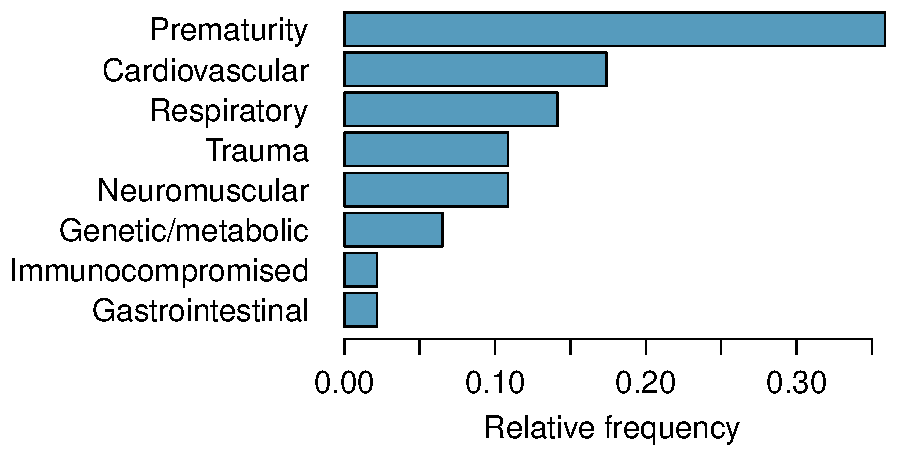
\includegraphics[width = 0.45\textwidth]{ch_summarizing_data/figures/eoce/antibiotic_use_children/antibiotic_use_children_bar}
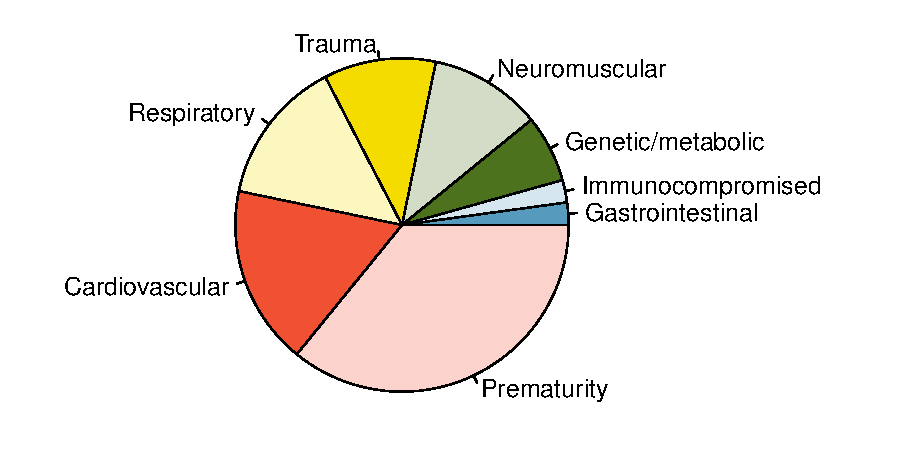
\includegraphics[width = 0.45\textwidth]{ch_summarizing_data/figures/eoce/antibiotic_use_children/antibiotic_use_children_pie}
\end{center}
\begin{parts}
\item What features are apparent in the bar plot but not in the pie chart?
\item What features are apparent in the pie chart but not in the bar plot?
\item Which graph would you prefer to use for displaying these categorical data?
\end{parts}
}{}

% 2

\eoce{\qt{Views on immigration\label{immigration}} 910 randomly sampled registered 
voters from Tampa, FL were asked if they thought workers who have illegally 
entered the US should be (i) allowed to keep their jobs and apply for 
US citizenship, (ii) allowed to keep their jobs as temporary guest workers 
but not allowed to apply for US citizenship, or (iii) lose their jobs and 
have to leave the country. The results of the survey by political ideology 
are shown below.\footfullcite{survey:immigFL:2012}
\begin{center}
\begin{tabular}{l l c c c c}
                        &                           & \multicolumn{3}{c}{\textit{Political ideology}} \\
\cline{3-5}
                        &                           & Conservative  & Moderate  & Liberal   & Total \\
\cline{2-6}
                        & (i) Apply for citizenship & 57            & 120       & 101       & 278 \\
                        & (ii) Guest worker         & 121           & 113       & 28        & 262 \\
\raisebox{1.5ex}[0pt]{\emph{Response}} & (iii) Leave the country    & 179       & 126       & 45        & 350 \\ 
                        & (iv) Not sure             & 15            & 4         & 1         & 20\\
\cline{2-6}
                        & Total                     & 372           & 363       & 175       & 910
\end{tabular}
\end{center}
\begin{parts}
\item What percent of these Tampa, FL voters identify themselves as conservatives?
\item What percent of these Tampa, FL voters are in favor of the citizenship option?
\item What percent of these Tampa, FL voters identify themselves as conservatives 
and are in favor of the citizenship option?
\item What percent of these Tampa, FL voters who identify themselves as 
conservatives are also in favor of the citizenship option? What percent of 
moderates share this view? What percent of liberals share this view?
\item Do political ideology and views on immigration appear to be independent? 
Explain your reasoning.
\end{parts}
}{}

% 3

\eoce{\qt{Views on the DREAM Act\label{dream_act_mosaic}} A random sample of registered 
voters from Tampa, FL were asked if they support the DREAM Act, a proposed law which would provide a path to citizenship for people brought illegally to the US as children.
The survey also collected information on the political ideology of the respondents. 
Based on the mosaic plot shown below, do views on the DREAM Act and  
political ideology appear to be independent? Explain your reasoning.
\footfullcite{survey:immigFL:2012}
\begin{center}
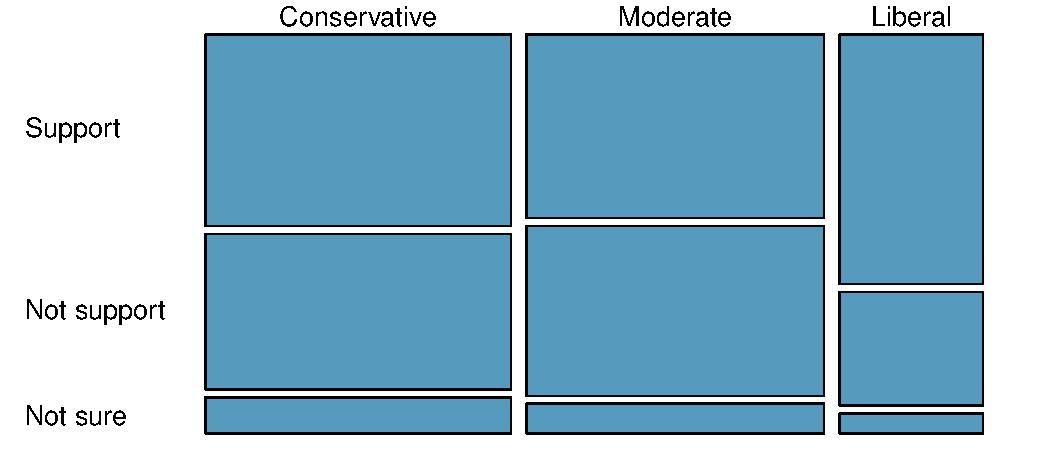
\includegraphics[width = 0.8\textwidth]{ch_summarizing_data/figures/eoce/dream_act_mosaic/dream_act_mosaic.pdf}
\end{center}
}{}

% 4

\eoce{\qt{Raise taxes\label{raise_taxes_mosaic}} A random sample of registered 
voters nationally were asked whether they think it's better to raise taxes 
on the rich or raise taxes on the poor. The survey also collected information 
on the political party affiliation of the respondents. Based on the mosaic 
plot shown below, do views on raising taxes and  
political affiliation appear to be independent? Explain your reasoning.
\footfullcite{survey:raiseTaxes:2015}
\begin{center}
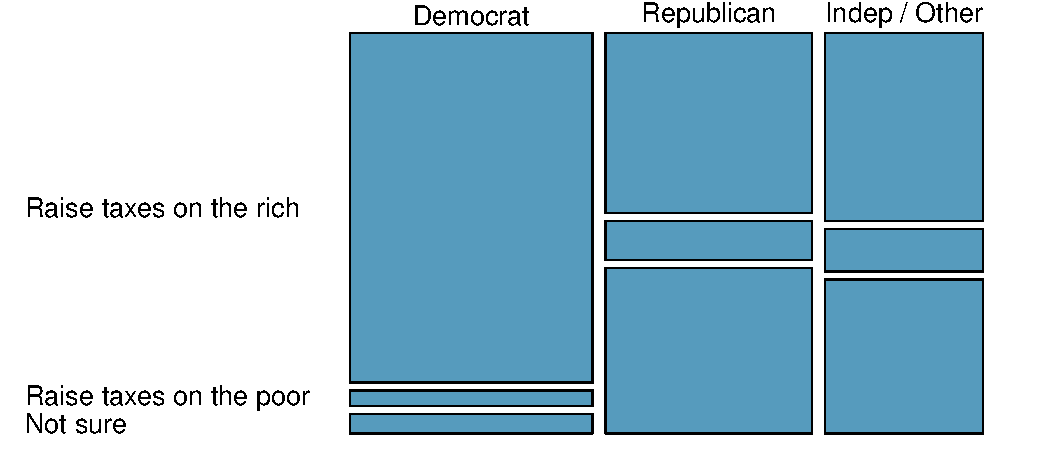
\includegraphics[width = 0.75\textwidth]{ch_summarizing_data/figures/eoce/raise_taxes_mosaic/raise_taxes_mosaic.pdf}
\end{center}
}{}
}





%___________________________________________
\section{Case study: malaria vaccine}
\label{caseStudyMalariaVaccine}

\begin{examplewrap}
\begin{nexample}{Suppose your professor splits the students in class into two groups: students on the left and students on the right. If $\hat{p}_{_L}$ and $\hat{p}_{_R}$ represent the proportion of students who own an Apple product on the left and right, respectively, would you be surprised if $\hat{p}_{_L}$ did not {exactly} equal $\hat{p}_{_R}$?}\label{classRightLeftSideApple}
While the proportions would probably be close to each other, it would be unusual for them to be exactly the same. We would probably observe a small difference due to {chance}.
\end{nexample}
\end{examplewrap}

\begin{exercisewrap}
\begin{nexercise}
If we don't think the side of the room a person sits on
in class is related to whether the person owns an Apple product,
what assumption are we making about the relationship between
these two variables?\footnotemark{}
\end{nexercise}
\end{exercisewrap}
\footnotetext{We would be assuming that these two variables
  are independent.}


\subsection{Variability within data}
\label{variabilityWithinData}

\index{data!malaria vaccine|(}

We consider a study on a new malaria vaccine
called PfSPZ.
In this study, volunteer patients were randomized
into one of two experiment groups:
14 patients received an experimental vaccine
or 6 patients received a placebo vaccine.
Nineteen weeks later, all 20 patients were exposed
to a drug-sensitive malaria virus strain;
the motivation of using a drug-sensitive strain
of virus here is for ethical considerations,
allowing any infections to be treated effectively.
The results are summarized in
Figure~\ref{malaria_vaccine_20_exp_summary},
where 9 of the 14 treatment patients remained free
of signs of infection while all of the~6 patients
in the control group patients showed some baseline
signs of infection.

\newcommand{\malariaAA}{5}
\newcommand{\malariaAB}{9}
\newcommand{\malariaAD}{14}
\newcommand{\malariaBA}{6}
\newcommand{\malariaBB}{0}
\newcommand{\malariaBD}{6}
\newcommand{\malariaDA}{11}
\newcommand{\malariaDB}{9}
\newcommand{\malariaDD}{20}
\newcommand{\malariaVIR}{0.357}
\newcommand{\malariaVIRPerc}{35.7\%}
\newcommand{\malariaPIR}{1.000}
\newcommand{\malariaPIRPerc}{100\%}
\newcommand{\malariaIRDiff}{0.643}
\newcommand{\malariaIRDiffPerc}{64.3\%}

\begin{figure}[ht]
\centering
\begin{tabular}{l l cc rr}
  & & \multicolumn{2}{c}{\var{outcome}} \\
  \cline{3-4}
  &  &  {infection} & {no infection} & Total & \hspace{3mm}  \\ 
  \cline{2-5}
  & {vaccine} &
      \malariaAA{} &
      \malariaAB{} &
      \malariaAD{} \\ 
  \raisebox{1.5ex}[0pt]{\var{treatment}}
  & {placebo} & 
      \malariaBA{} &
      \malariaBB{} &
      \malariaBD{} \\ 
  \cline{2-5}
  & Total & 
      \malariaDA{} &
      \malariaDB{} &
      \malariaDD{} \\ 
  \cline{2-5}
\end{tabular}
\caption{Summary results for the malaria vaccine experiment.}
\label{malaria_vaccine_20_exp_summary}
\end{figure}

\begin{exercisewrap}
\begin{nexercise}
Is this an observational study or an experiment?
What implications does the study type have on what can
be inferred from the results?\footnotemark{}
\end{nexercise}
\end{exercisewrap}
\footnotetext{The
  study is an experiment, as patients were randomly
  assigned an experiment group.
  Since this is an experiment, the results can be used
  to evaluate a causal relationship between the malaria
  vaccine and whether patients showed signs
  of an infection.}

In this study, a smaller proportion of patients
who received the vaccine showed signs of an infection
(\malariaVIRPerc{} versus \malariaPIRPerc{}).
However, the sample is very small,
and it is unclear whether the difference provides
\emph{convincing evidence} that the vaccine is
effective.

\D{\newpage}

\begin{examplewrap}
\begin{nexample}{Data scientists are sometimes called
    upon to evaluate the strength of evidence.
    When looking at the rates of infection for patients
    in the two groups in this study,
    what comes to mind as we try to determine whether
    the data show convincing evidence of a real difference?}
  \label{malaria_vaccine_20_what_is_convincing}
  The observed infection rates
  (\malariaVIRPerc{} for the treatment group versus
  \malariaPIRPerc{} for the control group)
  suggest the vaccine may be effective.
  However, we cannot be sure if the observed difference
  represents the vaccine's efficacy or is just from
  random chance.
  Generally there is a little bit of fluctuation
  in sample data, and we wouldn't expect the sample
  proportions to be \emph{exactly} equal,
  even if the truth was that the infection rates
  were independent of getting the vaccine.
  Additionally, with such small samples,
  perhaps it's common to observe such large differences
  when we randomly split a group due to chance alone!
\end{nexample}
\end{examplewrap}

Example~\ref{malaria_vaccine_20_what_is_convincing}
is a reminder that the observed outcomes in the data
sample may not perfectly reflect the true relationships
between variables since there is \term{random noise}.
While the observed difference in rates of infection
is large, the sample size for the study is small,
making it unclear if this observed difference represents
efficacy of the vaccine or whether it is simply due to
chance.
We label these two competing claims, $H_0$ and $H_A$,
which are spoken as ``H-nought'' and ``H-A'':
\begin{itemize}
\setlength{\itemsep}{0mm}
\item[$H_0$:] \textbf{Independence model.}
    The variables \var{treatment} and \var{outcome}
    are independent.
    They have no relationship, and the observed difference
    between the proportion of patients who developed
    an infection in the two groups, \malariaIRDiffPerc{},
    was due to chance.
\item[$H_A$:] \textbf{Alternative model.}
    The variables are \emph{not} independent.
    The difference in infection rates of
    \malariaIRDiffPerc{}
    was not due to chance,
    and vaccine affected the rate of infection.
\end{itemize}

What would it mean if the independence model,
which says the vaccine had no influence on the
rate of infection, is true?
It would mean 11~patients were going to
develop an infection \emph{no matter which group
they were randomized into},
and 9~patients would not develop an infection
\emph{no matter which group they were randomized
into}.
That~is, if the vaccine did not affect the rate
of infection, the difference in the infection rates
was due to chance alone in how the patients were
randomized.

Now consider the alternative model:
infection rates were influenced by whether a patient
received the vaccine or not.
If this was true, and especially if this influence
was substantial, we would expect to see some difference
in the infection rates of patients in the groups.

We choose between these two competing claims
by assessing if the data conflict so much with
$H_0$ that the independence model cannot be deemed
reasonable.
If this is the case, and the data support $H_A$,
then we will reject the notion of independence
and conclude there was discrimination.


\subsection{Simulating the study}
\label{simulatingTheStudy}

We're going to implement
\termsub{simulations}{simulation},
where we will pretend we know that the malaria
vaccine being tested does \emph{not} work.
Ultimately, we want to understand if the large
difference we observed is common in these
simulations.
If it is common, then maybe the difference
we observed was purely due to chance.
If it is very uncommon, then the possibility
that the vaccine was helpful seems more plausible.

Figure~\ref{malaria_vaccine_20_exp_summary}
shows that 11 patients developed infections and 9 did not.
For our simulation, we will suppose the infections
were independent of the vaccine and we were able to
\emph{rewind} back to when the researchers randomized
the patients in the study.
If we happened to randomize the patients differently,
we may get a different result in this hypothetical
world where the vaccine doesn't influence the infection.
Let's complete another \term{randomization} using
a simulation.

\D{\newpage}

In this \term{simulation}, we take 20 notecards to
represent the 20 patients, where we write down ``infection''
on 11 cards and ``no infection'' on 9 cards.
In this hypothetical world, we believe each patient
that got an infection was going to get it regardless
of which group they were in, so let's see what happens
if we randomly assign the patients to the treatment
and control groups again.
We thoroughly shuffle the notecards and deal 14 into
a \resp{vaccine} pile and 6 into a \resp{placebo} pile.
Finally, we tabulate the results, which are shown in
Figure~\ref{malaria_vaccine_20_exp_summary_rand_1}.

\begin{figure}[ht]
\centering
\begin{tabular}{l l cc rr}
  & & \multicolumn{2}{c}{\var{outcome}} \\
  \cline{3-4}
  &  &  {infection} & {no infection} & Total & \hspace{3mm}  \\ 
  \cline{2-5}
  treatment & {vaccine} & 7 & 7 & 14 \\ 
  (simulated) & {placebo} & 4 & 2 & 6 \\ 
  \cline{2-5}
  & Total & 11 & 9 & 20 \\
  \cline{2-5}
\end{tabular}
\caption{Simulation results, where any difference
    in infection rates is purely due to chance.}
\label{malaria_vaccine_20_exp_summary_rand_1}
\end{figure}

\begin{exercisewrap}
\begin{nexercise}
\label{malaria_vaccine_20_exp_summary_rand_1_diff}
What is the difference in infection rates between
the two simulated groups in
Figure~\ref{malaria_vaccine_20_exp_summary_rand_1}?
How does this compare to the observed
\malariaIRDiffPerc{} difference
in the actual data?\footnotemark{}
\end{nexercise}
\end{exercisewrap}
\footnotetext{$4 / 6 - 7 / 14 = 0.167$
  or about 16.7\% in favor of the vaccine.
  This difference due to chance is much smaller than the
  difference observed in the actual groups.}


\subsection{Checking for independence}

We computed one possible difference under the
independence model in Guided
Practice~\ref{malaria_vaccine_20_exp_summary_rand_1_diff},
which represents one difference due to chance.
While in this first simulation, we physically dealt
out notecards to represent the patients,
it is more efficient to perform this simulation
using a computer.
Repeating the simulation on a computer, we get another
difference due to chance:
\begin{align*}
\frac{2}{\malariaBD{}} - \frac{9}{\malariaAD{}} = -0.310
\end{align*}
And another:
\begin{align*}
\frac{3}{\malariaBD{}} - \frac{8}{\malariaAD{}} = -0.071
\end{align*}
And so on until we repeat the simulation enough times
that we have a good idea of what represents the
\emph{distribution of differences from chance alone}.
Figure~\ref{malaria_rand_dot_plot} shows a stacked plot
of the differences found from 100 simulations,
where each dot represents a simulated difference between
the infection rates (control rate minus treatment rate).

\begin{figure}[ht]
  \centering
  \Figure{0.85}{malaria_rand_dot_plot}
  \caption{A stacked dot plot of differences from
      100 simulations produced under the independence model,
      $H_0$, where in these simulations infections are
      unaffected by the vaccine.
      Two of the 100 simulations had a difference of
      at least \malariaIRDiffPerc{}, the difference observed
      in the study.}
  \label{malaria_rand_dot_plot}
\end{figure}

Note that the distribution of these simulated differences
is centered around 0.
We simulated these differences assuming that the independence
model was true, and under this condition,
we expect the difference to be near zero with some random
fluctuation, where \emph{near} is pretty generous in this
case since the sample sizes are so small in this study.

\begin{examplewrap}
\begin{nexample}{How often would you observe a difference
    of at least \malariaIRDiffPerc{} (\malariaIRDiff{})
    according to Figure~\ref{malaria_rand_dot_plot}?
    Often, sometimes, rarely, or never?}
  It appears that a difference of at least
  \malariaIRDiffPerc{} due to chance alone would only
  happen about 2\% of the time according to
  Figure~\ref{malaria_rand_dot_plot}.
  Such a low probability indicates a rare event.
\end{nexample}
\end{examplewrap}

\D{\newpage}

The difference of \malariaIRDiffPerc{} being
a rare event suggests two possible interpretations
of the results of the study:
\begin{itemize}
  \setlength{\itemsep}{0mm}
  \item[$H_0$] \textbf{Independence model.}
      The vaccine has no effect on infection rate,
      and we just happened to observe a difference
      that would only occur on a rare occasion.
  \item[$H_A$] \textbf{Alternative model.}
      The vaccine has an effect on infection rate,
      and the difference we observed was actually due to
      the vaccine being effective at combatting malaria,
      which explains the large difference
      of~\malariaIRDiffPerc{}.
\end{itemize}
Based on the simulations, we have two options.
(1)~We conclude that the study results do not provide
strong evidence against the independence model.
That is, we do not have sufficiently strong evidence
to conclude the vaccine had an effect in this
clinical setting.
(2)~We conclude the evidence is sufficiently strong
to reject $H_0$ and assert that the vaccine was useful.
When we conduct formal studies, usually we reject the
notion that we just happened to observe a rare
event.\footnote{This reasoning does not generally extend
    to anecdotal observations.
    Each of us observes incredibly rare events every day,
    events we could not possibly hope to predict.
    However, in the non-rigorous setting of anecdotal
    evidence, almost anything may appear to be a rare event,
    so the idea of looking for rare events in day-to-day
    activities is treacherous.
    For example, we might look at the lottery:
    there was only a 1 in 292 million chance that the
    Powerball numbers for the largest jackpot in history
    (January 13th, 2016) would be (04, 08, 19, 27, 34)
    with a Powerball of (10),
    but nonetheless those numbers came up!
    However, no matter what numbers had turned up,
    they would have had the same incredibly rare odds.
    That is, \emph{any set of numbers we could have
    observed would ultimately be incredibly rare}.
    This type of situation is typical of our daily lives:
    each possible event in itself seems incredibly rare,
    but if we consider every alternative, those outcomes
    are also incredibly rare.
    We should be cautious not to misinterpret such
    anecdotal evidence.}
So in this case, we reject the independence model in favor
of the alternative.
That is, we are concluding the data provide strong evidence
that the vaccine provides some protection against malaria
in this clinical setting.

\index{data!malaria vaccine|)}

One field of statistics, statistical inference, is built
on evaluating whether such differences are due to chance.
In statistical inference, data scientists evaluate which
model is most reasonable given the data.
Errors do occur, just like rare events, and we might choose
the wrong model.
While we do not always choose correctly, statistical
inference gives us tools to control and evaluate how
often these errors occur.
In Chapter~\ref{foundationsForInference},
we give a formal introduction to the problem of model
selection.
We spend the next two chapters building a foundation
of probability and theory necessary to make that
discussion rigorous.



{\exercisesheader{}

% 1

\eoce{\qt{Side effects of Avandia\label{randomization_avandia}} Rosiglitazone is the 
active ingredient in the controversial type~2 diabetes medicine Avandia and has 
been linked to an increased risk of serious cardiovascular problems such as 
stroke, heart failure, and death. A common alternative treatment is pioglitazone, 
the active ingredient in a diabetes medicine called Actos. In a nationwide 
retrospective observational study of 227,571 Medicare beneficiaries aged  
65 years or older, it was found that 2,593 of the 67,593 patients using 
rosiglitazone and 5,386 of the 159,978 using pioglitazone had serious 
cardiovascular problems. These data are summarized in the contingency 
table below. \footfullcite{Graham:2010}
\begin{center}
\begin{tabular}{ll  cc c} 
                                &   & \multicolumn{2}{c}{\textit{Cardiovascular problems}} \\
\cline{3-4} 
                                    &               & Yes   & No        & Total \\
\cline{2-5}
\multirow{2}{*}{\textit{Treatment}} & Rosiglitazone & 2,593 & 65,000    & 67,593 \\
                                    & Pioglitazone  & 5,386 & 154,592   & 159,978 \\
\cline{2-5}
                                    & Total         & 7,979 & 219,592   & 227,571
\end{tabular}
\end{center}
\begin{parts}
\item Determine if each of the following statements is true or false. If false, explain why. \textit{Be careful:} The reasoning may be wrong even if the statement's conclusion is correct. In such cases, the statement should be considered false.
\begin{subparts}
\item Since more patients on pioglitazone had cardiovascular problems (5,386 vs. 2,593), we can conclude that the rate of cardiovascular problems for those on a pioglitazone treatment is higher.
\item The data suggest that diabetic patients who are taking rosiglitazone are more likely to have cardiovascular problems since the rate of incidence was (2,593 / 67,593 = 0.038) 3.8\% for patients on this treatment, while it was only (5,386 / 159,978 = 0.034) 3.4\% for patients on pioglitazone.
\item The fact that the rate of incidence is higher for the rosiglitazone group proves that rosiglitazone causes serious cardiovascular problems.
\item Based on the information provided so far, we cannot tell if the difference between the rates of incidences is due to a relationship between the two variables or due to chance.
\end{subparts}
\item What proportion of all patients had cardiovascular problems?
\item If the type of treatment and having cardiovascular problems were independent, about how many patients in the rosiglitazone group would we expect to have had cardiovascular problems?
\item We can investigate the relationship between outcome and treatment in this study using a randomization technique.  While in reality we would carry out the simulations required for randomization using statistical software, suppose we actually simulate using index cards. In order to simulate from the independence model, which states that the outcomes were independent of the treatment, we write whether or not each patient had a cardiovascular problem on cards, shuffled all the cards together, then deal them into two groups of size 67,593 and 159,978. We repeat this simulation 1,000 times and each time record the number of people in the rosiglitazone group who had cardiovascular problems. Use the relative frequency histogram of these counts to answer (i)-(iii).
\end{parts}
\begin{minipage}[c]{0.5\textwidth}
\begin{subparts}
\item What are the claims being tested?
\item Compared to the number calculated in part (b), which would provide more support for the alternative hypothesis,  \textit{more} or \textit{fewer} patients with cardiovascular problems in the rosiglitazone group?
\item What do the simulation results suggest about the relationship between taking rosiglitazone and having cardiovascular problems in diabetic patients?
\end{subparts}
\end{minipage}
\begin{minipage}[c]{0.5\textwidth}
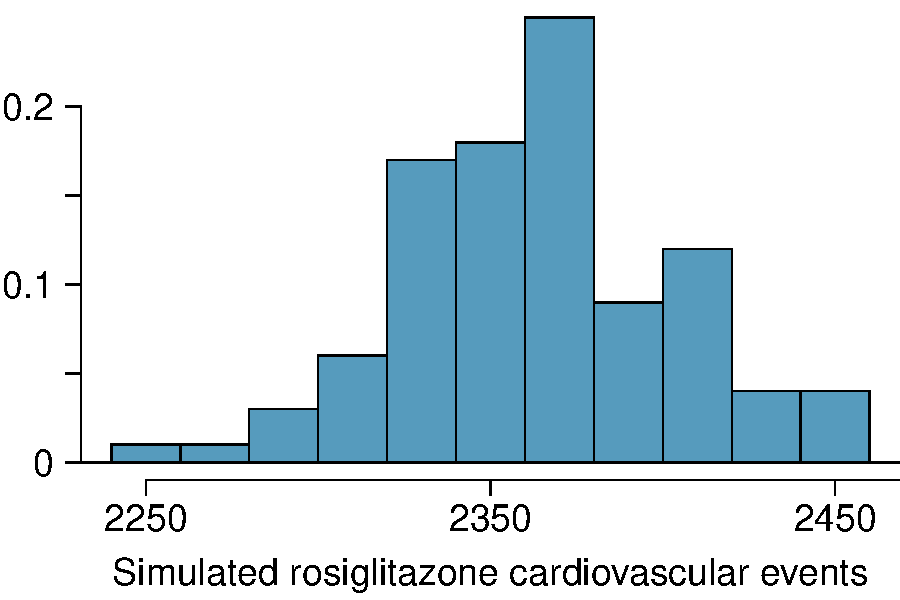
\includegraphics[width = \textwidth]{ch_summarizing_data/figures/eoce/randomization_avandia/randomization_avandia.pdf} \\
\end{minipage}
}{}

% 2

\eoce{\qt{Heart transplants\label{randomization_heart_transplants}} The Stanford 
University Heart Transplant Study was conducted to determine whether an 
experimental heart transplant program increased lifespan. Each patient 
entering the program was designated an official heart transplant candidate, 
meaning that he was gravely ill and would most likely benefit from a new heart. 
Some patients got a transplant and some did not. The variable \texttt{transplant} 
indicates which group the patients were in; patients in the treatment group got a 
transplant and those in the control group did not. Of the 34 patients in the 
control group, 30 died. Of the 69 people in the treatment group, 45 died. Another 
variable called \texttt{survived} was used to indicate whether or not the patient 
was alive at the end of the study. \footfullcite{Turnbull+Brown+Hu:1974}
\begin{center}
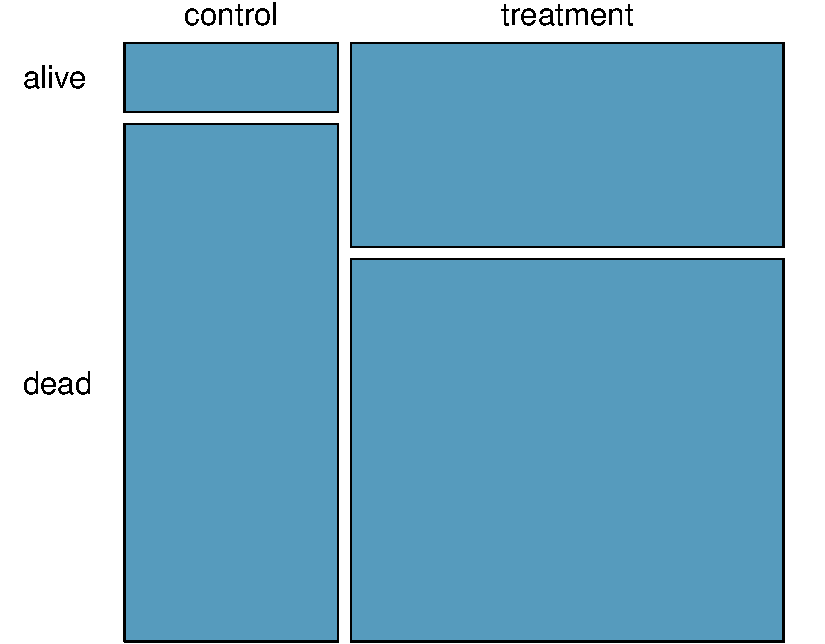
\includegraphics[width= 0.48\textwidth]{ch_summarizing_data/figures/eoce/randomization_heart_transplants/randomization_heart_transplants_mosaic.pdf}
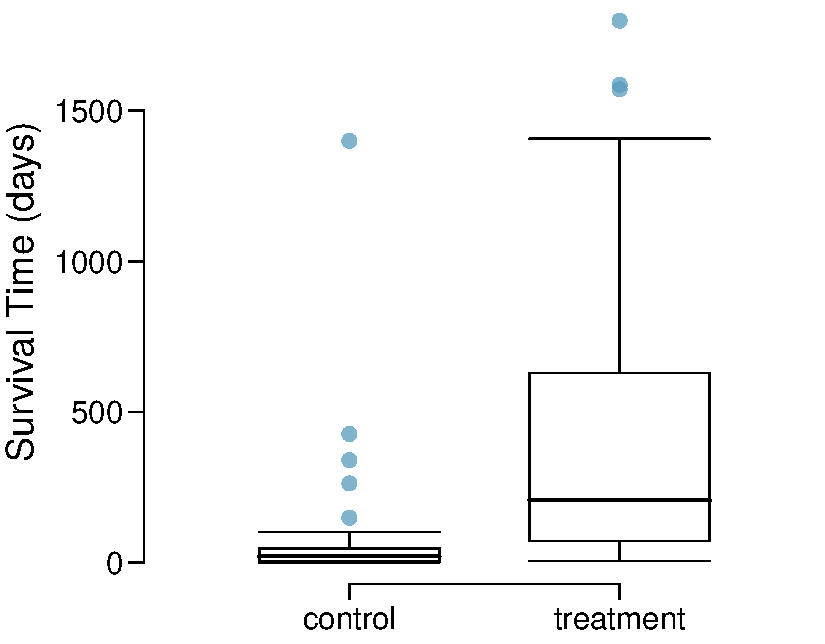
\includegraphics[width= 0.48\textwidth]{ch_summarizing_data/figures/eoce/randomization_heart_transplants/randomization_heart_transplants_box.pdf}
\end{center}
\begin{parts}
\item Based on the mosaic plot, is survival independent of whether or not the 
patient got a transplant? Explain your reasoning.
\item What do the box plots below suggest about the efficacy (effectiveness) of the heart transplant treatment.
\item What proportion of patients in the treatment group and what proportion of 
patients in the control group died?
\item One approach for investigating whether or not the treatment is effective 
is to use a randomization technique.
\begin{subparts}
\item What are the claims being tested?
\item The paragraph below describes the set up for such approach, if we were 
to do it without using statistical software. Fill in the blanks with a number 
or phrase, whichever is appropriate.
\begin{adjustwidth}{2em}{2em}
We write \textit{alive} on \rule{2cm}{0.5pt} cards representing patients who were 
alive at the end of the study, and \textit{dead} on \rule{2cm}{0.5pt} cards 
representing patients who were not. Then, we shuffle these cards and split them 
into two groups: one group of size \rule{2cm}{0.5pt} representing treatment, and 
another group of size \rule{2cm}{0.5pt} representing control. We calculate the 
difference between the proportion of \textit{dead} cards in the treatment and 
control groups (treatment - control) and record this value. We repeat this 100 
times to build a distribution centered at \rule{2cm}{0.5pt}. Lastly, we calculate 
the fraction of simulations where the simulated differences in proportions are 
\rule{2cm}{0.5pt}. If this fraction is low, we conclude that it is unlikely to 
have observed such an outcome by chance and that the null hypothesis should 
be rejected in favor of the alternative.
\end{adjustwidth}
\item What do the simulation results shown below suggest about the effectiveness 
of the transplant program?
\end{subparts}
\end{parts}
\begin{center}
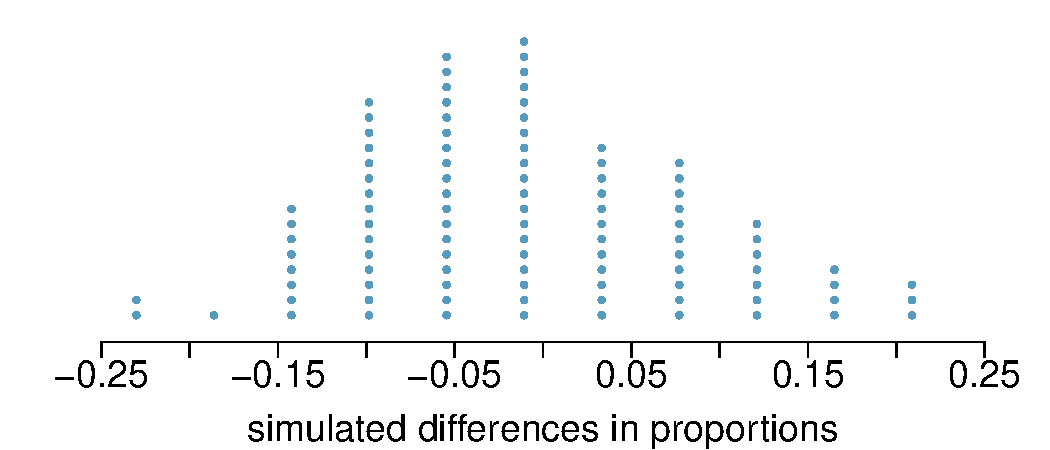
\includegraphics[width= 0.6\textwidth]{ch_summarizing_data/figures/eoce/randomization_heart_transplants/randomization_heart_transplants_rando.pdf}
\end{center}
}{}
}
